\documentclass[12pt, letterpaper]{article}
\usepackage[titletoc,title]{appendix}
\usepackage{color}
\usepackage{booktabs}
\usepackage[usenames,dvipsnames,svgnames,table]{xcolor}
\definecolor{dark-red}{rgb}{0.75,0.10,0.10} 
\usepackage[margin=1in]{geometry}
\usepackage[linkcolor=dark-red,
colorlinks=true,
urlcolor=blue,
pdfstartview={XYZ null null 1.00},
pdfpagemode=UseNone,
citecolor={dark-red},
pdftitle={Agenda Bias}]{hyperref}

\usepackage[resetlabels,labeled]{multibib}
\newcites{SI}{SI References}
\usepackage{natbib}

\usepackage{float}

\usepackage{geometry} % see geometry.pdf on how to lay out the page. There's lots.
\geometry{letterpaper}               % This is 8.5x11 paper. Options are a4paper or a5paper or other... 
\usepackage{graphicx}                % Handles inclusion of major graphics formats and allows use of 
\usepackage{amsfonts,amssymb,amsbsy}
\usepackage{amsxtra}
\usepackage{verbatim}
\setcitestyle{round,semicolon,aysep={},yysep={;}}
\usepackage{setspace}		     % Permits line spacing control. Options are \doublespacing, \onehalfspace
\usepackage{sectsty}		     % Permits control of section header styles
\usepackage{lscape}
\usepackage{fancyhdr}		     % Permits header customization. See header section below.
\usepackage{url}                     % Correctly formats URLs with the \url{} tag
\usepackage{fullpage}		%1-inch margins
\usepackage{multirow}
\usepackage{rotating}
\setlength{\parindent}{3em}
\usepackage{booktabs}
\usepackage{longtable}
\usepackage[T1]{fontenc}
\usepackage{bm}
\usepackage{libertine}

\usepackage{chngcntr}

%This section double-spaces & makes footnotes the same size as normal text.
\usepackage{footmisc}
\setlength{\footnotesep}{\baselineskip}
\makeatother
\renewcommand{\footnotelayout}{\normalsize \doublespacing}


% Caption
\usepackage[hang, font=small,skip=0pt, labelfont={bf}]{caption}
%\captionsetup[subtable]{font=small,skip=0pt}
\usepackage{subcaption}

% tt font issues
% \renewcommand*{\ttdefault}{qcr}
\renewcommand{\ttdefault}{pcr}

\setcounter{page}{0}

\usepackage{lscape}
\renewcommand{\textfraction}{0}
\renewcommand{\topfraction}{0.95}
\renewcommand{\bottomfraction}{0.95}
\renewcommand{\floatpagefraction}{0.40}
\setcounter{totalnumber}{5}
\makeatletter
\providecommand\phantomcaption{\caption@refstepcounter\@captype}
\makeatother

\title{Measuring Agendas, and Positions on Agendas}

\author{Gaurav Sood\thanks{Gaurav can be reached at \href{mailto:gsood07@gmail.com}{\footnotesize{\texttt{gsood07@gmail.com}}}} \and Andy Guess\thanks{Andy can be reached at \href{mailto:guess@nyu.edu}{\texttt{guess@nyu.edu}}}\vspace{.5cm}}

\begin{document}
\maketitle
\thispagestyle{empty}

\begin{center}
\vspace{.5cm}\textbf{NB:} Preliminary draft. Please do not cite without permission.\vspace{1.5cm}
\end{center}
\begin{comment}
	
setwd(paste0(basedir, "issue_ideology/ms/"))
tools::texi2dvi("issue_ideology.tex", pdf=TRUE,clean=TRUE)
setwd(basedir)

\end{comment}

\begin{abstract}
\noindent Variation in agendas and positions on agendas are independently important. The former explains the kinds of issues people think are important, and the latter potentially explains people's positions on the issues. In this paper, we estimate variation on both these dimensions. To do this, we first estimate a supervised topic model using the bill labels from the Policy Agendas Project. Then within each of the topics, we estimate a model of slant using congressional speech as training data. Using this method, we scale 255 news programs across 50 television channels using original, and closed captions transcripts from these shows. We find large systematic variation in broad agendas of news media, and positions on those agendas.  
\end{abstract}

\textbf{Keywords}: Media bias, ideology, supervised topic models, agenda bias

\clearpage
\doublespace
Media are our `window to the world.' What the media cover, and how they cover it, affects what we know about the world \citep{jerit2006citizens}, influences which issues we think are important \citep{mccombs1972agenda, behr1985, iyengar1993news}, and shapes how we think about those issues \citep[for e.g.][]{iyengar1990framing, iyengar1996framing}. For instance, exogenous shocks to the amount of news coverage of disasters affect how much money is donated to disaster victims \citep{eisensee2007news}. By the same token, who people think is responsible for crime depends on whether the media frames the issue episodically or thematically \citep{iyengar1989citizens}. Suffice to say that both, what issues are covered in the news, and how they are covered matters.

Recent changes in news media---transition from mass media to new media---and the public, notably greater partisan animus \citep{iyengar2012affect}, have raised worries about a particular kind of media bias---partisan bias. In the past decade, numerous studies have estimated partisan bias in the media using two broad strategies. Some scholars have estimated ideology of the media as a function of shared phrases used by the media and the members of congress, using extant measures of politicians' ideology to impute scores for the media \citep[see, for e.g.,][]{groseclose2005, gentzkow2010}. Other set of scholars have exploited differences in audiences of various media outlets, using a structural model of consumption behavior to identify ideological location of news sources \citep[see, for e.g.,][]{barbera2014follow, gentzkow2011}. 

Both these ways of estimating partisan bias, however, potentially conflate at least two distinct pathologies --- what the media covers (the agenda) and how it covers it. In this paper, we attempt to pry apart these two important kinds of variation. We do so by first estimating a supervised topic model using a corpora of labeled Congressional Bills from the Policy Agendas Project \citep{baumgartner2003policy}. We then use the model to predict the topics covered in various news outlets. We find significant variation across media outlets but also significant correlation in topical coverage across time---news media cover the same issue at about the same time. We then predict the Congressional speech corpora to estimate the partisan slant of each topic. Building on work by \citet{puglisi2011being} and \citet{larcinese2011partisan}, we use this information to create a measure of partisan slant based on agendas of media outlets. And then as a last step, we partition our congressional speech corpora into topical domains and estimate slant within each domain. We then use this to estimate variation in how the same topic is covered across outlets.  

\section*{Why Distinguish Between Agendas and Positions on Agendas?}

Consider a news organization that covers illegal immigration extensively. Without knowing anything more about the news organization, one would be hard pressed to say whether the news organization is for or against greater expenditure on border security. The news outlet could be Univision or the Fox News Channel or anything in between. For there is no necessary correlation between prioritizing an issue and position on the issue.  Media organizations on all sides of the issue can think that an issue is important, and spend a great deal of time covering it. 

Not only is the distinction between agendas and positions on agendas conceptually important, it is also important for understanding the consequences of exposure to media. For, exposure to an agenda may simply cause people to think a particular issue is important, and not affect their position on the issue. For instance, local media's coverage of crime may make both Republicans and Democrats more concerned about crime, but may not change the viewers' opinions about how to solve crime. In fact, the long-held commonly expressed worry about media's power has to do with how exposure to media informs how important people think an issue is, not media's ability to influence people's positions on the issues. In Cohen's oft-quoted words, ``the press may not be successful much of the time in telling people what to think, but it is stunningly successful in telling its readers what to think about'' \citep{cohen1963press}.

Affecting the importance of an issue can have important downstream consequences. In particular, agenda biases can affect partisan preferences. This is so because people believe that different parties are better at dealing with different issues---that the parties `own' certain issues \citep{petrocik1996issue}. For instance, people think that the Democratic Party is more competent at managing problems related to welfare, health care, and labor, while the Republicans are perceived as more competent on defense \citep{petrocik1996issue, goggin2015}. And `priming' issues owned by a particular party can advantage that party \citep{petrocik1996issue, petrocik2003issue}. \citet{puglisi2011being, larcinese2011partisan} build on that insight to describe variation in agenda of New York Times, and on economic issues by various newspapers, respectively. 

Lastly, for very plausible reasons, agenda biases can have a larger influence people's preferences than exposure to explicit positions. The reasoning is straightforward--- it is easy for people to discern the ideology based on explicit positions, and discount information that is uncongenial to them. However, it is likely that people are less aware of biases in agendas and their power to shape opinions. Selecting what information to reveal can thus produce bias even with rational agents \citep[for relevant formal theoretic accounts, see][]{anderson2012media, bernhardt2008political}.

Besides the potential effects of agenda biases on preferences on public preferences, agenda biases likely also affect policy making. \citet{egan2013partisan}, for instance, postulates that agendas of parties not just reflect stereotypes about competence that the parties can exploit, but also parties' legislative priorities. By focusing on a particular issue, a groundswell for dealing with that particular issue may be created. In all, distinguishing between agendas and positions on agendas may lead to a better understanding of effects of media.

Aside from reasons to do with better understanding effects of media by coding `treatment' appropriately, differentiating between agenda and positions on the agenda may also be useful for creating better models of the economics of the media industry. A long literature in political science suggests that for a variety of reasons, some people are more interested in some issues than others \citep{iyengar2008selective, krosnick1990government, krosnick1995public}. For instance, partly perhaps due to self-interest, older people are more interested (and informed) about issues to do with Medicare, and younger people are more informed about issues to do with student-lending and health insurance for the young. Interest in an issue can outstrip interest in listening to a particular position on the issue \citep{iyengar2008selective}. To pursue the example of Medicare further, Americans over the age of 65 may be interested in all information to do with Medicare, not just, say the position of the Republican party. All in all, there exist a variety of important reasons to distinguish between agendas and positions on the agendas.

\section*{Expectations About (Co)-Variation in Agendas and Positions on Agendas}

There are competing conjectures about whether or not we should see much variation in agendas of news outlets. At one end, there are good reasons to think that the agendas of media are highly constrained by real world events and politicians' agendas. At the other end, there are reasons to think that the media have ample opportunity to be entrepreneurial about the agendas, and have ample incentives to take advantage of those opportunities. We investigate either end of the pool sequentially, fleshing out the logic and other relevant hypothesis that stem from these postulates. 

If we assume that the media organizations (actors, outlets) do not act as independent political players trying to influence the politics of the country, the account of media's agenda degenerates to following what the people want. This in turn may in turn may mean covering appropriate real world events, and following the congressional agenda. The congressional agenda in turn is influenced by the majority party \citep{gailmard2007negative}. 

The real world events may, however, dictate both the congress' and the media's agenda. In fact, one possibility is simply that the news media (and to some extent Congress) go from covering one `salient' real world event to another \citep[]{boydstun2013making, birkland1998focusing}. (What we mean by salient is theoretically debatable but appears to be widely agreed upon within the polity --- mass murders in the U.S. for instance are nearly universally acknowledged as newsworthy these days.) For instance, when the mass murders happen in South Carolina.\footnote{See \href{https://en.wikipedia.org/wiki/Charleston_church_shooting}{https://en.wikipedia.org/wiki/Charleston\_church\_shooting}.}, the media focus on that event. And then some time later, another thing happens, and the news media changes its focus to that event. 

The prediction from such kinds of models is that the media's agendas ought to be broadly similar. And that over-time correlation in agendas ought to be high. This also means that any ideological bias ought to come from how the events are covered. For instance, while covering the shooting, Fox News may emphasize that had the pastor been armed, the tragedy could have been averted. On the other hand, MSNBC may emphasize the racial angle of the shooting. Or the Fox News may cover the racialization of the shooting by MSNBC. Or the MSNBC may decry the lack of discussion of race in shooting on conservative channels. The point is that the difference is less to do with what is covered and more to do with how it is covered. 

But between these events, there are also fallow periods and other news programming that is less focused on current events. In those fallow periods, and on news programs less focused on covering current events, there is an opportunity for pursuing independent agendas. And we conjecture that the news outlets take this opportunity to cover issues that are important to them for one reason or another. For instance, some may pursue an issue because it is personally important to people in the editorial board. Or because the news media outlet is interested in building a groundswell of support for an issue it thinks can help their preferred party. Or for some other reason entirely. 

In all, there exist good reasons to think both of the points are true---that media's agendas are largely constrained but do allow some opportunity for entrepreneurship. We empirically assess the extent to which the expectations hold. But before we do so, we describe the data, the measures, and our analytical strategy.

\section*{Data and Measures}

Our first goal is to estimate the political agenda of the news media. In particular, we want to classify the topical content of transcripts of television news shows, and articles from variety of online news outlets. To do so, we start by training a supervised topic model based on bill labels produced by the Policy Agendas Project (PAP) \citep{baumgartner2003policy}. To accomplish this, we download the entire corpora of nearly 27,000 congressional bills and PAP's labels and other miscellanea for these bills. PAP labels congressional bills as belonging to one of 20 major issue areas, ranging from Macroeconomics to Immigration to Environment to Defense. Each of these major issue areas are further sub-divided into sub-topics. (See ~\ref{si2} for all the subtopic labels per topic.) For instance, Macroeconomics is further subdivided into Inflation, Prices, and Interest Rates, Unemployment Rate, National Budget and Debt, etc. These sub-topics are informative, especially with regards to partisanship---for instance, Republicans are liable to speak more about budget deficits than Democrats, even though they may be no less interested in talking about Macroeconomics more generally --- but to get a better sense of coverage of broad agendas, we start by estimating a model of how major topic areas relate to the text of the bills. The coherence of the topics in PAP labels is not particularly high. For instance, the topic `Law, Crime, and Family Issues' spans from organized crime to child support.  So, we also learn a model of 90 selected (with enough support) minor topic labels.

To estimate the model of how topic areas relate to text, we start with the standard text preprocessing stems of lemmatizing, removing `stop words', and punctuation, losing all words less than 2 characters long, and converting all the words to lower case. We further assume a 1-, 2- Markov model of language, storing just frequency of bigrams and trigrams and removing order information. Since we plan to use the data to predict ideology of the news data, we take an additional step of removing bi- and tri-grams that either don't exist in our news database or occur than 20,000 times. (See \citet{gentzkow2010} and \citet{MartinYurukoglu2014}, among others who have used similar assumptions in modeling similar text.) Next, we split the data into a test-set (20\%) and a training-set (80\%). On the training set, we use Support Vector Machine (SVM) classifier \citep{guyon2002gene} to model the relationship between classes and phrases. 
\begin{align*} 
& \left\lVert w \right\rVert^2 + C\sum_{i=1}^{m} \xi_i\\
& \text{   subject to: } y_i(w \cdot x_i + b) \ge 1 - \xi_i, \xi_i \ge 0
\end{align*}

The out of sample accuracy for the model is approximately 80\%. Figure ~\ref{major_conf} plots the out-of-sample confusion matrix of actual and predicted labels when we predict major topics, and figure ~\ref{minor_conf} the boxplot of accuracy scores for minor topics. \ref{si_top20} shows the top 20 predictors of each of the topics.  

\begin{figure}[H]
\centering
\caption{Out of Sample Confusion Matrix for Major Topics}\label{major_conf}
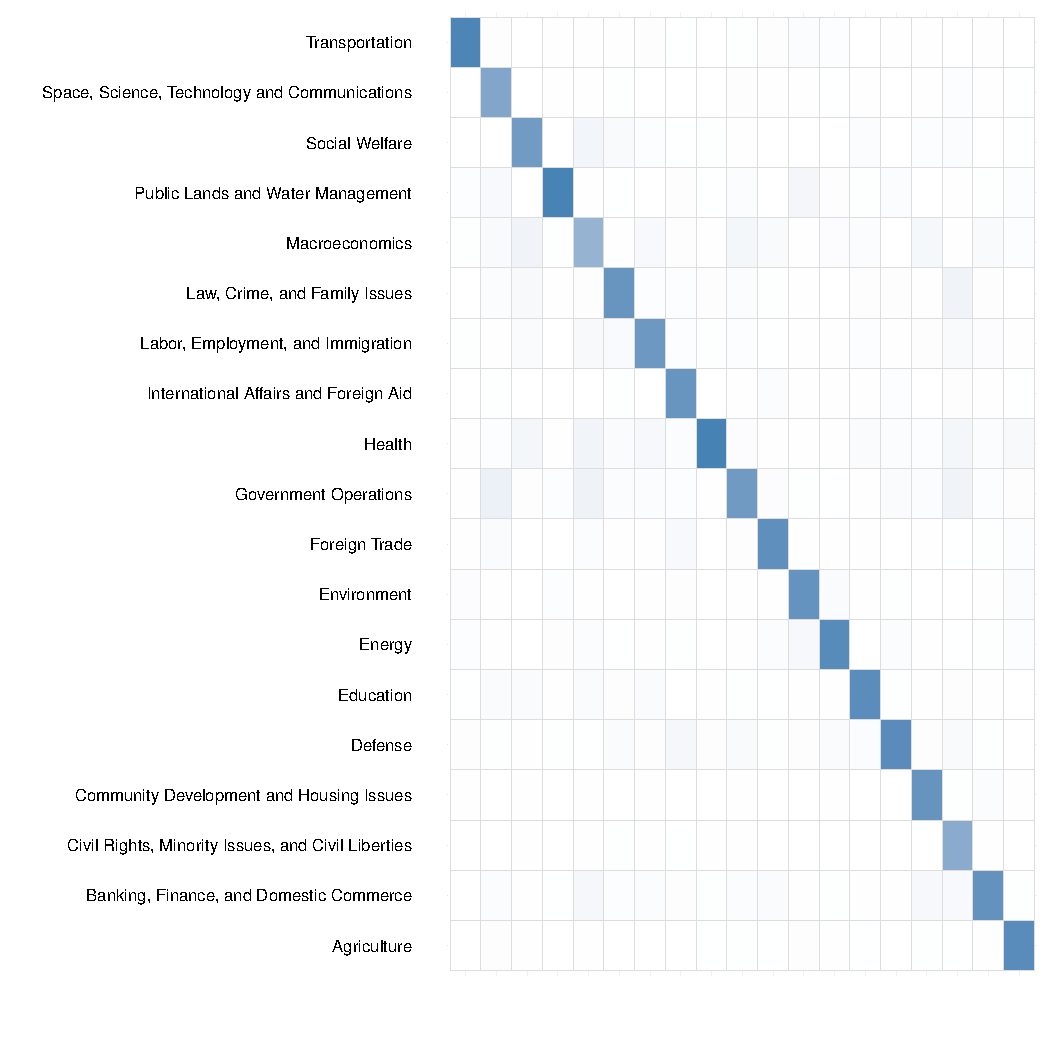
\includegraphics[width=.75\textwidth]{../figs/conf_matrix_topic.pdf}
\end{figure}

\begin{figure}[H]
\centering
\caption{Distribution of Out of Sample Accuracy for Minor Topics}\label{minor_conf}
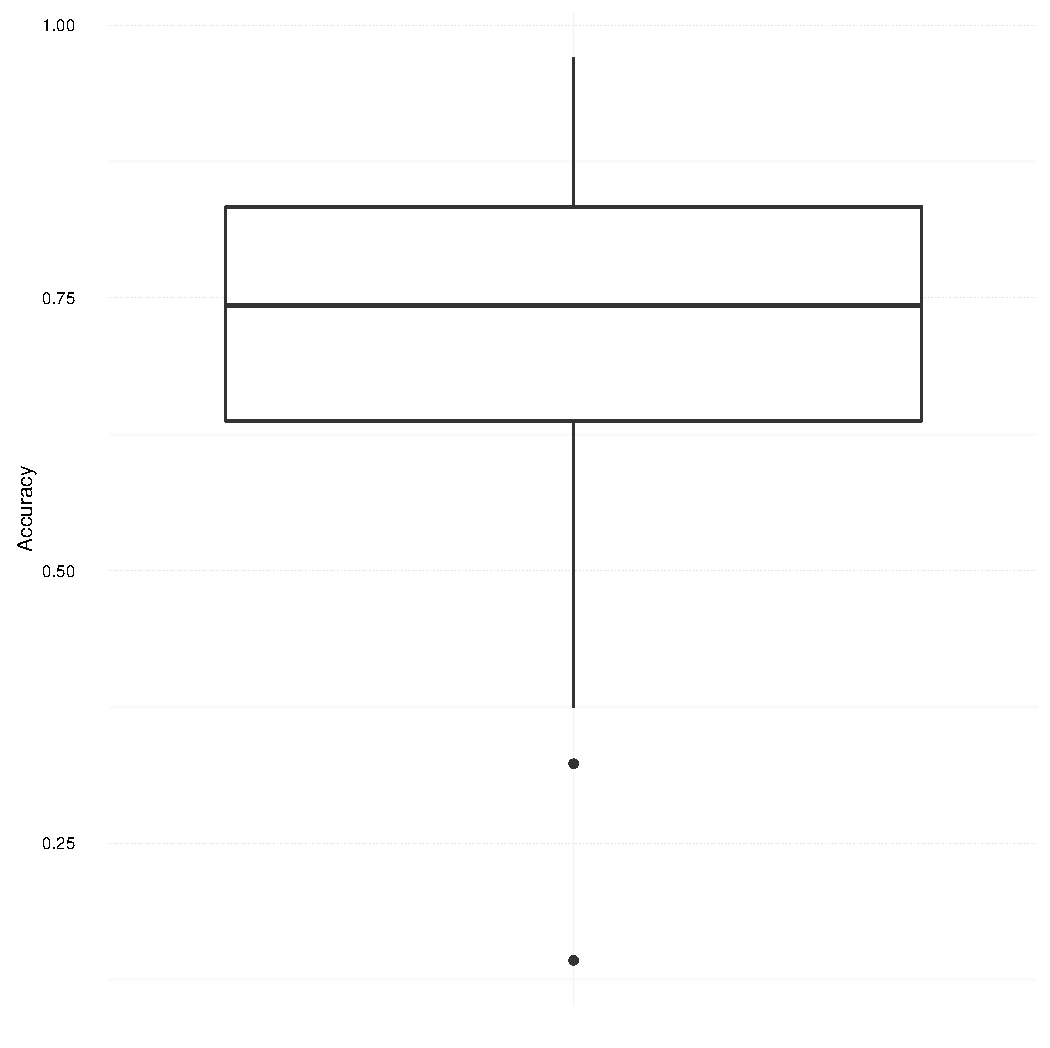
\includegraphics[width=.75\textwidth]{../figs/conf_matrix_topic_all.pdf}
\end{figure}

To estimate the relationship between parties and emphasis on different topical areas, we use three training sets---congressional speech corpora for the 111th and the 112th congress, party manifestos of the two major parties over the past 20 years, and the 100 recent most Facebook wall posts of members of congress (as of October 2015).\footnote{We downloaded the congressional speech data using a \href{https://github.com/soodoku/speech-learn/blob/master/scripts/capitol_speech.py}{python module} that interfaces with the CapitolWords API by the Sunlight Foundation. We accessed manifesto data via the manifestos project \citep{manifesto2015}. For the Facebook data, we relied on R package, \href{https://github.com/pablobarbera/Rfacebook}{RFacebook}, an R Client for the Facebook API.} We preprocessed the data as before. Next, using the model we estimate above, we predict all the congressional corpora. We next calculate the extent to which an average Republican talks more about a topic than an average Democrat by predicting the topics of all the speech and the Facebook wall posts corpora. We synthesize the information as the extent to which Republicans speak about it more often than Democrats. Everything is rescaled from -1 to 1 where -1 is where Republicans speak about it all the time, and Democrats never, 0 reflecting a case where Democrats and Republicans speak about it equally and 1 where only Democrats speak on a topic.

Lastly, we predict news data. Our textual news data originates from several sources. And importantly, it focuses on television news, still a major source of political information for most Americans \citep{chaffee1996americans}.\footnote{For more recent data, see \href{http://www.americanpressinstitute.org/publications/reports/survey-research/how-americans-get-news/}{How Americans Get Their News}, a 2014 report by the American Press Institute, and results of the \href{http://www.gallup.com/poll/163412/americans-main-source-news.aspx}{2013 Gallup Survey}.} We acquired broadcast transcripts from Fox News, CNNfn (CNN's now-defunct financial news network), CNN International, and MSNBC from NewsBank, a provider of full-text archives from a range of news sources, from 2000 to 2012. We supplemented this data with text transcripts from the Internet Archive (2009-2012) and the University of California, Los Angeles Closed Caption archive (LACC, 2006--2012) covering shows from CNBC, CNN, Current TV, Fox News, and MSNBC. In total we have data on more than 50 television channels, and 255 shows, e.g. NBC Nightly News, O'Reilly Factor, Countdown, CBS Evening News etc. Finally, we were able to download the text of stories posted to \href{CNN.com}{http://cnn.com} (2000--2014) and \href{MSNBC.com}{http://msnbc.com} (2010--2014) websites. We subset the data to shows with at least 100 transcripts each. And again we preprocess the text data --- stemming, removing stop-words and punctuation etc. as before. The table in the Appendix (see ~\ref{si1}) provides details on the number of transcripts in our combined data by show as well as the date range for each.

Our next goal is to predict slant within agendas. For this purpose we use speech data from the 111th and the 112th Congress.\footnote{The time period for our media data is much longer and ideally we want to predict only contemporaneous data to account for changes in cleavages, phrases used to fight the same ideological battles, etc. over time. We plan to do that in the next iteration.} While our eventual aim is to predict slant among all topics, we for now limits ourselves to the salient issue of immigration. Within the congressional speech classified as to be on the topic of immigration, we estimate a model predicting party of the speaker, once again using SVM within Vowpal Wabbit. 

\section*{Results}

\subsection*{Variation in Agendas}
If all the media organizations prayed from the same book---current events (and similar biases on what is news worthy) and congressional agenda---we would expect the distribution of topics within media to be broadly the same. On the other hand, if the media organizations exercised discretion in what to cover or had different preferences, we would expect heterogeneity in the frequency with which various topics are covered. To study the question, we looked at the frequency with which various topics are covered in various news channels. We define the quantity of interest as proportion of net coverage devoted to a topic. Alternate definitions---for e.g., total coverage of an issue---are reasonable but sensitive to frequency of news program, etc.\footnote{On television, there is a large opportunity cost for covering a topic. In a medium like newspapers or the Internet, a news media organization can cover multiple issues in depth as space is much less constrained.}

For illustration, we limit ourselves to television channel-level aggregates. For focusing attention on crucial details, we limit ourselves to five topics, chosen mostly for variety and importance---immigration, education and macroeconomics. Figure ~\ref{var_agendas} plots the distribution of the topics across channels. As we can see, there is healthy variation. 

However, this healthy variation hides a fair bit of co-variation. Figure ~\ref{over_time} shows topical coverage across channels across time. As we can see, coverage co-varies a bit. In fact, the average across-time correlation in proportion of coverage devoted to an issue across the eight channels is .47. For a noisy series, this is a pretty strong correlation. Average correlation in changes in coverage across issues --- with month as a unit (the optimal unit of time likely varies by issue)---also has a pulse---it is .33. This suggests that switches in focus across time are somewhat systematic, likely a consequence of exogenous factors.

\begin{figure}[H]
\centering
\caption{Over Time Variation in Agendas}\label{over_time}
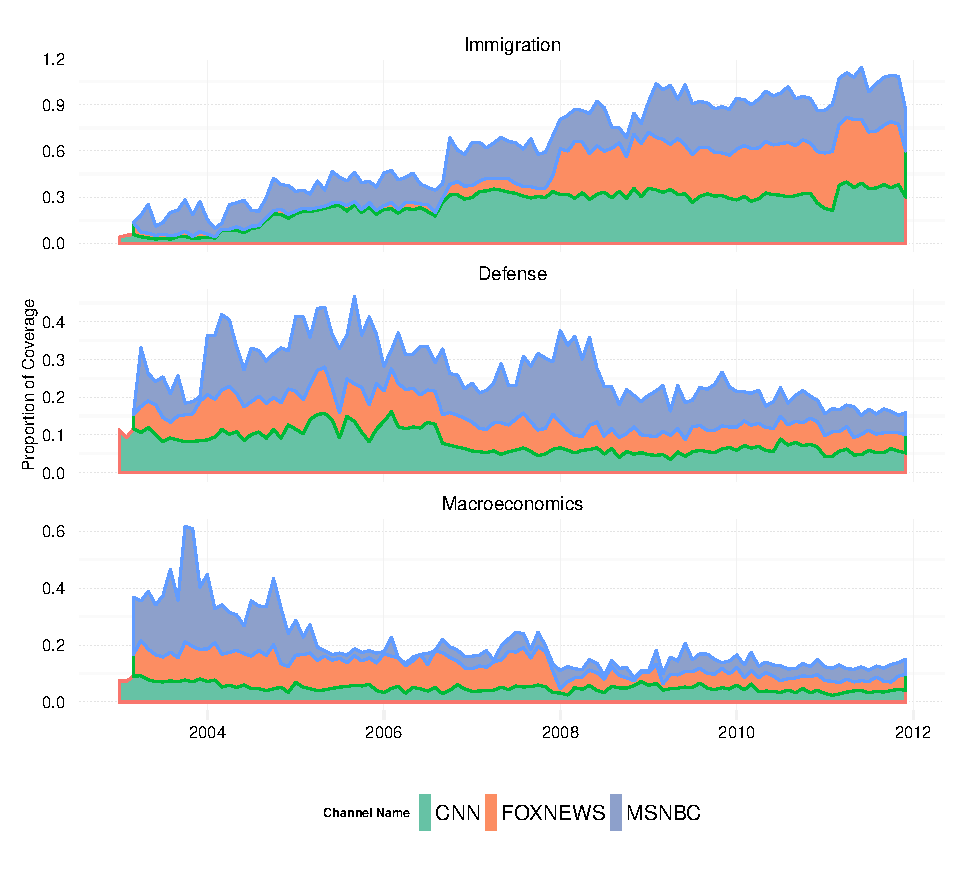
\includegraphics[width=1\textwidth]{../figs/topic_channel_time.pdf}
\end{figure}

\subsection*{Partisanship of Agendas}

Next, we estimate the partisanship of the agendas. But before we present the results, a couple of caveats about interpretation. The current estimates only come from predicting Congressional speech text, which, as we note, is vastly constrained. We plan to discern partisanship of the agendas through `speech' on less constrained media, such as manifestos and Facebook data, in the next iteration of the paper. Second, the Policy Agenda Project major topics are exceedingly crude and we pool over over much meaningful variation.

After adjusting for different numbers of Democrats and Republicans, the data show that the share of Republican speech on an issue doesn't ever exceed or lag the speech by Democrats by more than 15\%. Figure ~\ref{partisan_issue} shows share of Republican (Democrat) speech on topics. There are some expected patterns in the data. Republicans speak more than Democrats on immigration, while Democrats speak more than Republicans on civil rights issues. 

\begin{figure}[H]
\centering
\caption{Partisanship of Agendas}
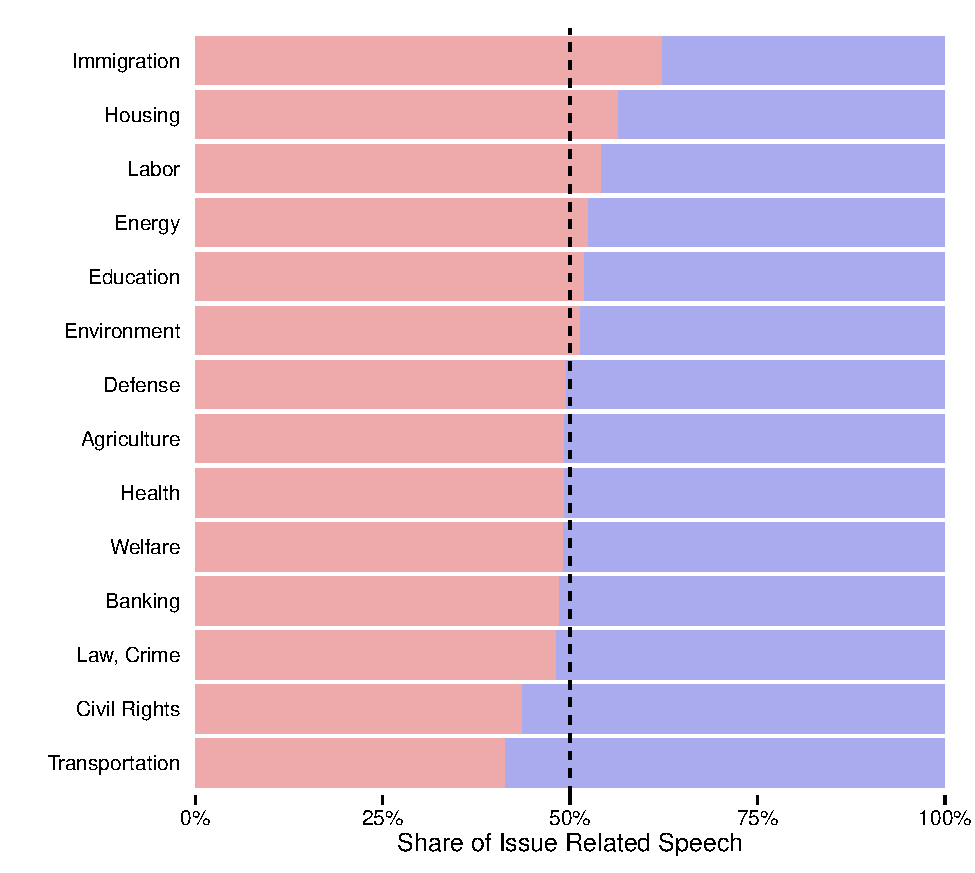
\includegraphics[width=.75\textwidth]{../figs/partisan_issue.pdf}\label{partisan_issue}
\end{figure}

\begin{figure}[H]
\centering
\caption{Partisanship of Agendas Over Time: Macro-economics}
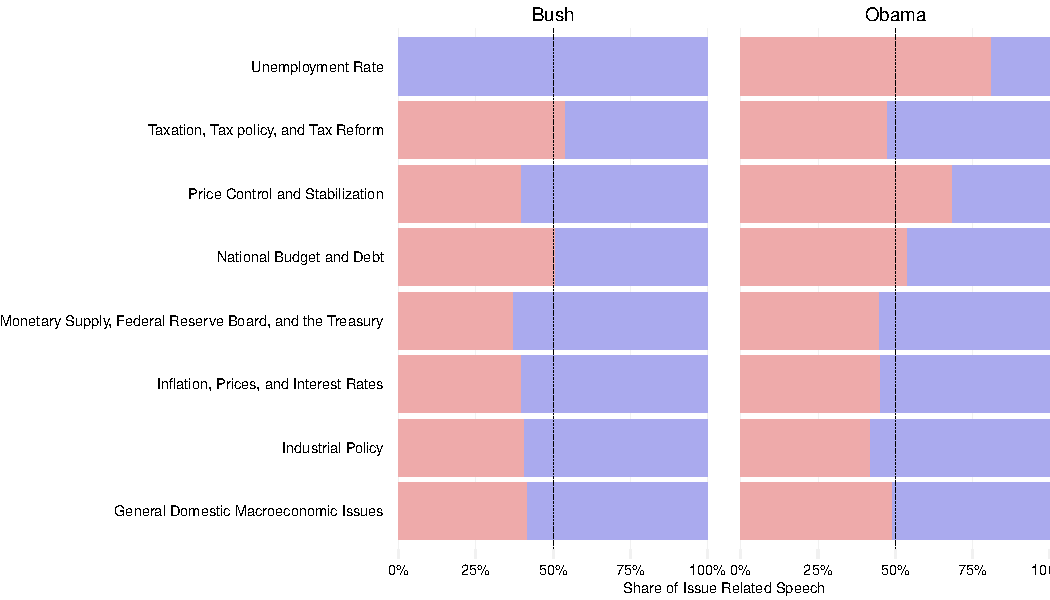
\includegraphics[width=.75\textwidth]{../figs/macro_by_obama.pdf}\label{partisan_issue}
\end{figure}

\begin{figure}[H]
\centering
\caption{Partisanship of Agendas Over Time: Defense}
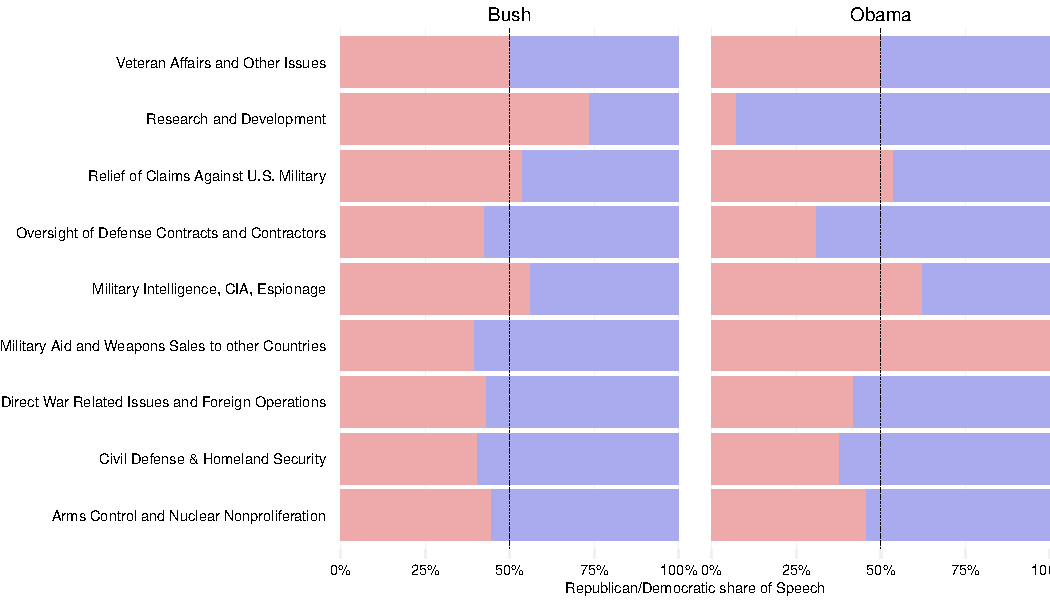
\includegraphics[width=.75\textwidth]{../figs/mil_by_obama.pdf}\label{partisan_issue}
\end{figure}

\subsection*{Partisan Agendas}

Next, we scale partisanship of shows by their agendas. Again, before we discuss the results, we would like to issue a couple of caveats about interpretation. Even if a show focuses on a particular issue that advantages a party, it doesn't mean that the reasons the show's editors focused on the issue were partisan. External factors, unrelated to partisanship, may be to blame. For instance, the New York Times may cover poverty more often because it is founded in an urban environment with a high proportion of people suffering from poverty. So any partisan agenda may be accidental. Second, we only estimate bias in topics included in the Policy Agendas Projects. This is not a complete (though likely a large) universe of topics. Figure ~\ref{pagenda} presents distribution of partisanship of shows (extent to which the agenda across the Policy Agendas Topics is Democratic) nested within channels. The overall variation is compressed, partly as a result of choice of crude topics, none of which have an overwhelming partisan slant, and partly because the shows don't focus exclusively on the most partisan topics. Despite these issues, you can see that the median of Fox News is to the right of MSNBC, CNN, and other network channels.  

\begin{figure}[H]
\centering
\caption{Partisanship of Agendas}\label{pagenda}
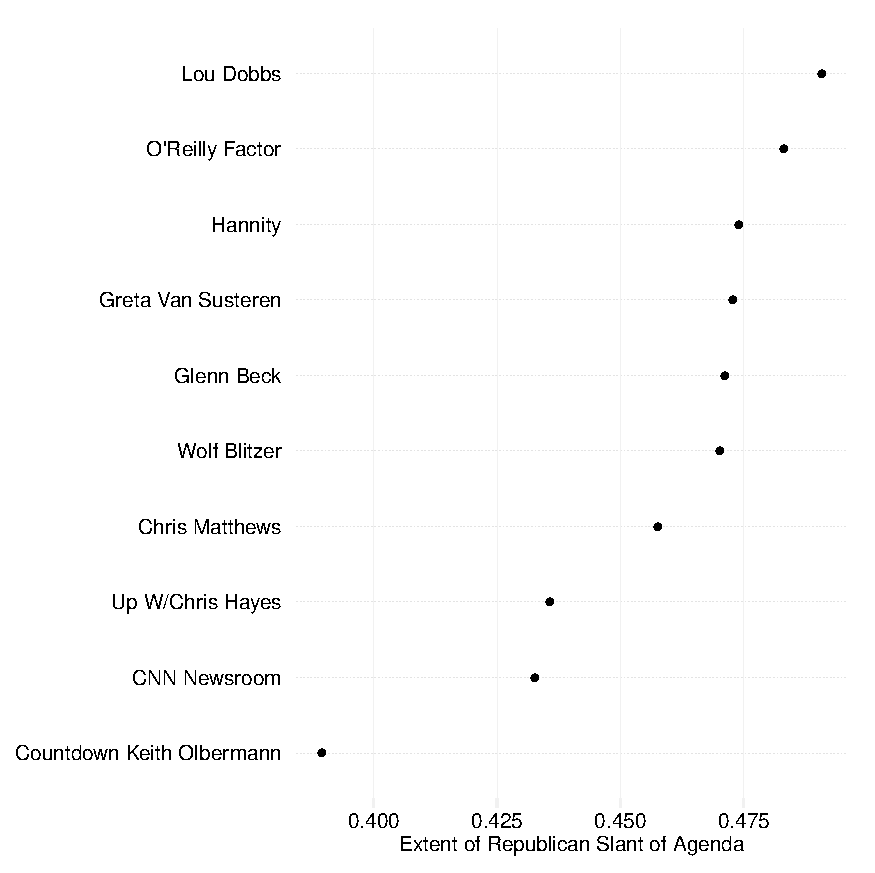
\includegraphics[width=.75\textwidth]{../figs/partisanship_of_agenda.pdf}
\end{figure}

\subsection*{Positions within Agendas}
Lastly, we focus on estimating positions within agendas. For now, we limit ourselves to just one topic---civil rights. As we discuss, we use congressional speech on the topic of immigration as training data. Using a model trained on the congressional data, we impute the partisanship of various television shows on the issue. We cluster the estimates by channel. Figure ~\ref{pcivil} shows the extent to which the slant is Democratic for each show on civil rights. Again Fox News median is to the right but there is a lot of overlap across channels.

\begin{figure}[H]
  \begin{subfigure}[t]{0.48\textwidth}
   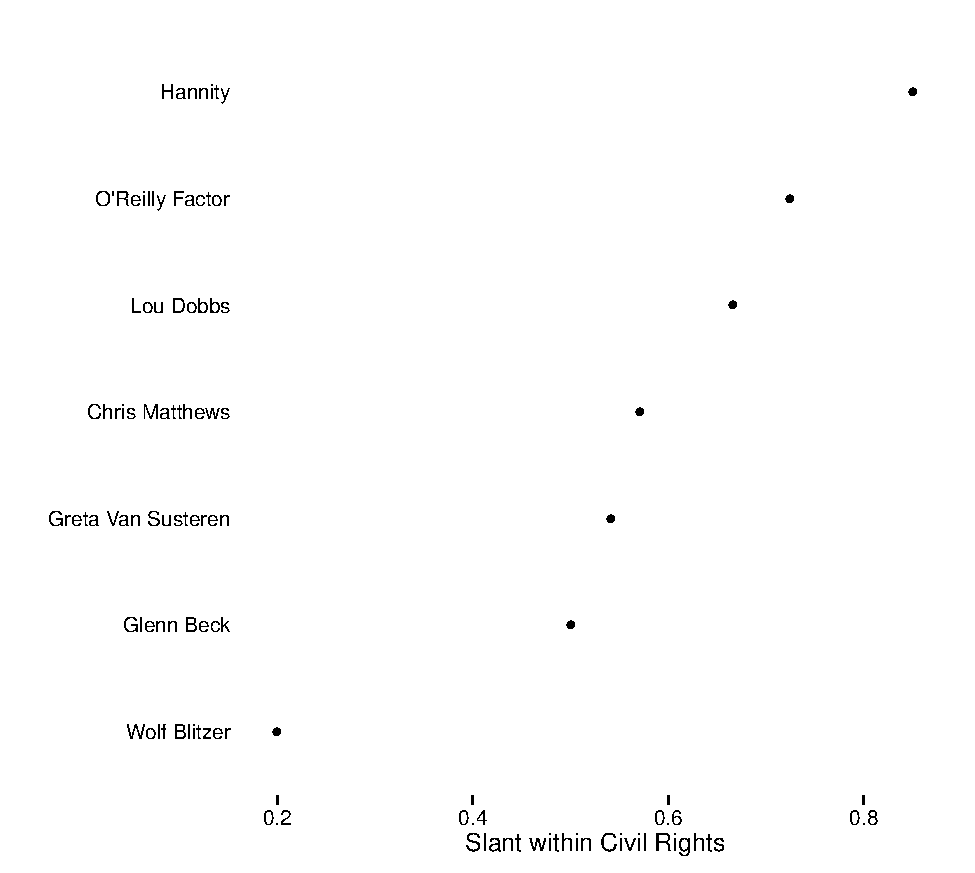
\includegraphics[width=\textwidth]{../figs/civil_prefs.pdf}
    \end{subfigure}
     \hfill
    \begin{subfigure}[t]{0.48\textwidth}
    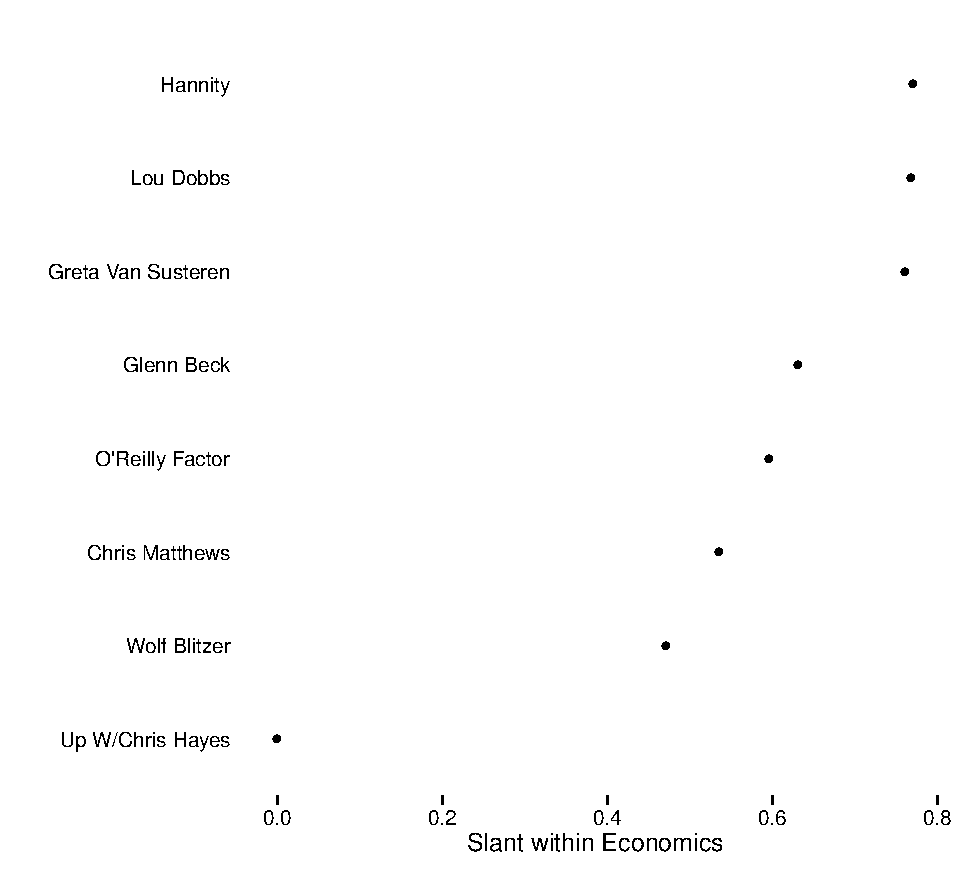
\includegraphics[width=\textwidth]{../figs/econ_prefs.pdf}
    \end{subfigure}
\end{figure}


\section*{Discussion}
The power of the agenda has been extensively discussed in political science. And forms basis of some work on measuring media bias \citep[see for instance,]{larcinese2011partisan}. In fact, the most general model of thinking about media bias is to posit a neutral source and then observe whether different media organizations selectively cover various issues. This forms the basis of research by \citep{baum2008new} who show that editorial judgments about placement of various news items is affected by ideology. We extend the research here, creating a supervised topic model based on Policy Agenda Topics, estimating partisanship of the agendas using political speech as training data, and then using both to describe variation in agendas and variation in slant within agendas. Our research contributes to the media effects literature in creating more nuanced measures that allow us to better measure media's political consequences. 

Our research also contributes to understanding on ideological scaling of media sources. Many recent attempts to scale ideology of news sources have relied on labeled political speech as training data to model the relationship between words and ideology \citep{groseclose2005, gentzkow2010}. However, language similarly can be driven by agendas that politicians pursue as much as positions on those agendas. What are the implications of our research for the measurement of ideological slant using congressional speech data as training data for building one model for relationship between words and ideology? There are potentially a couple. As we note above, language similarly can be driven by agendas that politicians pursue as much as positions on those agendas. Thus, the agendas of congress and media likely have to be largely concordant for models trained on congressional speech to yield valid indicators of differences in positions on issues. Secondly, and perhaps more importantly, media's ideology has also to be uni-dimensional. If media's positions on issues lie on more than one-dimension, congressional speech as training data to recover estimates of a generic ideological scale may not be enough. The model may still yield valid scores along the dimension of conflict spanned by congress, but it may not be enough.

Like others, we struggle with how we define a topic. To call something a topic doesn't make it a coherent entity. And a careful exegesis of Policy Agendas Projects labels for bills suggests that conceptual coherence of many of the major topic labels is debatable. In the next iteration of the paper, we plan to focus on more coherent minor topic labels in the Policy Agendas Project. But even doing so leaves open many questions. For even within a subtopic of taxation, there are a variety of policy issues. For instance, estate tax, corporate tax, etc. And that strikes us as a reasonable next step.

\clearpage

\bibliographystyle{apsr}
\bibliography{mediabias}

\clearpage
\appendix
\renewcommand{\thesection}{SI \arabic{section}}
\renewcommand\thetable{\thesection.\arabic{table}}  
\renewcommand\thefigure{\thesection.\arabic{figure}}
\counterwithin{figure}{section}


\begin{center}
\Large{Supporting Information}
\end{center}

\nocitesec{*}

\section{Summary of the Media Data}
\label{si1}
Our text data originates from several sources. Here we summarize the number of transcripts in our combined data by show, as well as the specific data source and date range for each.
\scriptsize
% latex table generated in R 3.2.2 by xtable 1.7-4 package
% Sun Oct 11 00:19:02 2015
{\scriptsize
\begin{longtable}{llllr}
\caption{Summary of the network, date range, and number of transcripts for each show in the text data.} \\ 
  \hline
Show & Network & From & To & \# of Transcripts \\ 
  \hline
1600 Pennsylvania Avenue & MSNBC & 11/05/2008 & 04/03/2009 & 108 \\ 
  ABC News Good Morning America & ABC & 07/03/2009 & 09/12/2012 & 2685 \\ 
  ABC World News David Muir & ABC & 02/19/2011 & 09/10/2012 & 277 \\ 
  ABC World News Diane Sawyer & ABC & 12/21/2009 & 09/13/2012 & 1549 \\ 
  ABC World News Now & ABC & 07/03/2009 & 09/12/2012 & 2043 \\ 
  ABC World News Saturday & ABC & 02/10/2007 & 08/20/2011 & 175 \\ 
  ABC World News Sunday & ABC & 12/20/2009 & 02/21/2011 & 468 \\ 
  ABCs World News Charles Gibson & ABC & 07/02/2009 & 12/18/2009 & 216 \\ 
  Abrams Report & MSNBC & 07/03/2007 & 08/29/2008 & 1249 \\ 
  Ahead of the Curve & CNN & 12/19/2000 & 04/03/2001 & 1908 \\ 
  All In Chris Hayes & MSNBC &  &  & 163 \\ 
  AM Wake Up Call & CNN & 06/27/2011 & 01/03/2012 & 260 \\ 
  America Live & FOXNEWS & 02/01/2010 & 09/12/2012 & 733 \\ 
  American Morning & CNN & 04/22/2003 & 12/30/2011 & 13544 \\ 
  American Morning Paula Zahn & CNN & 01/07/2002 & 04/21/2003 & 5231 \\ 
  American Morning: Wake Up Call & CNN & 06/27/2011 & 12/09/2011 & 119 \\ 
  Americas Election Hq & FOXNEWS & 04/22/2008 & 01/02/2009 & 180 \\ 
  Americas News HQ & FOXNEWS & 07/03/2011 & 09/09/2012 & 1162 \\ 
  Americas Newsroom & FOXNEWS & 07/03/2009 & 09/12/2012 & 836 \\ 
  Anderson Cooper & CNN & 07/03/2009 & 09/13/2012 & 9861 \\ 
  Andrea Mitchell Reports & MSNBC & 07/07/2009 & 09/12/2012 & 781 \\ 
  Anthony Bourdain Parts Unknown & CNN & 04/14/2013 & 03/02/2014 & 120 \\ 
  Around the World & CNN & 02/25/2013 & 02/07/2014 & 440 \\ 
  Asia Tonight & CNN & 05/14/2001 & 09/10/2001 & 360 \\ 
  Beltway Boys & FOXNEWS & 01/29/2005 & 12/15/2007 & 199 \\ 
  Big Story & FOXNEWS & 01/19/2004 & 12/20/2007 & 11673 \\ 
  Biz & CNN & 06/05/2003 & 09/20/2004 & 988 \\ 
  Biz Asia & CNN & 05/01/2001 & 09/11/2001 & 326 \\ 
  Breaking News & CNN & 04/04/2001 & 12/10/2013 & 5708 \\ 
  Buchanan \& Press & MSNBC & 04/03/2003 & 11/25/2003 & 158 \\ 
  Bulls \& Bears & FOXNEWS & 07/04/2009 & 09/08/2012 & 169 \\ 
  Burden of Proof & CNN & 04/05/2001 & 10/06/2001 & 409 \\ 
  CBS Evening News & CBS & 07/04/2009 & 09/10/2012 & 2239 \\ 
  CBS Evening News Katie Couric & CBS & 07/02/2009 & 06/04/2011 & 1085 \\ 
  CBS Evening News Russ Mitchell & CBS & 07/12/2009 & 01/02/2012 & 173 \\ 
  CBS Evening News Scott Pelley & CBS & 06/08/2011 & 09/12/2012 & 696 \\ 
  CBS Morning News & CBS & 07/03/2009 & 09/12/2012 & 1647 \\ 
  CBS News Sunday Morning & CBS & 07/05/2009 & 09/09/2012 & 764 \\ 
  CBS This Morning & CBS & 01/10/2012 & 09/12/2012 & 350 \\ 
  CNN Election Center & CNN & 02/19/2008 & 12/25/2008 & 177 \\ 
  CNN Money Morning & CNN & 06/06/2003 & 09/20/2004 & 624 \\ 
  CNN Newsroom & CNN & 07/02/2009 & 09/13/2012 & 6653 \\ 
  CNN Presents & CNN & 08/30/2009 & 08/26/2012 & 502 \\ 
  CNN Saturday Morning & CNN & 07/04/2009 & 03/10/2012 & 253 \\ 
  CNN Sunday Morning & CNN & 07/05/2009 & 03/11/2012 & 145 \\ 
  CNN in Session & CNN & 09/28/2011 & 11/08/2011 & 261 \\ 
  CNN: Special Investigations Unit & CNN & 01/20/2007 & 10/16/2011 & 278 \\ 
  CNNs Amanpour & CNN & 09/21/2009 & 03/07/2014 & 691 \\ 
  Campbell Brown & CNN & 06/03/2009 & 07/21/2010 & 664 \\ 
  Capital Gang & CNN & 04/07/2001 & 06/25/2005 & 225 \\ 
  Cashin in & FOXNEWS & 07/04/2009 & 09/08/2012 & 259 \\ 
  Cavuto on Business & FOXNEWS & 07/06/2009 & 09/08/2012 & 207 \\ 
  Cenk Uygur & MSNBC & 01/25/2011 & 02/29/2012 & 286 \\ 
  Chris Matthews & MSNBC & 07/02/2009 & 09/13/2012 & 3344 \\ 
  Connect the World & CNN & 01/27/2010 & 03/07/2014 & 1055 \\ 
  Connie Chung Tonight & CNN & 06/24/2002 & 03/19/2003 & 187 \\ 
  Countdown & MSNBC & 04/10/2003 & 03/28/2011 & 4192 \\ 
  Crossfire & CNN & 04/05/2001 & 03/07/2014 & 1447 \\ 
  Daily Rundown & MSNBC & 01/11/2010 & 09/13/2012 & 1283 \\ 
  Deborah Norville Tonight & MSNBC & 01/21/2004 & 01/13/2005 & 228 \\ 
  Diplomatic License & CNN & 07/07/2001 & 11/10/2006 & 267 \\ 
  Dolans Unscripted & CNN & 11/10/2003 & 09/20/2004 & 745 \\ 
  Dr. Drew & CNN & 04/04/2011 & 03/06/2014 & 648 \\ 
  Dylan Ratigan Show & MSNBC & 01/14/2010 & 08/29/2012 & 707 \\ 
  Early Edition & CNN & 01/04/2000 & 03/02/2001 & 2868 \\ 
  Early Start & CNN & 12/16/2013 & 03/07/2014 & 230 \\ 
  Early Start Ashleigh Banfield \& Zoraida Sambolin & CNN & 01/02/2012 & 08/08/2012 & 315 \\ 
  Early Start John Berman \& Zoraida Sambolin & CNN & 08/09/2012 & 12/13/2013 & 1046 \\ 
  Ed Show & MSNBC & 07/03/2009 & 09/13/2012 & 4219 \\ 
  Election Center & CNN & 03/25/2008 & 11/14/2008 & 668 \\ 
  Erin Burnett Out Front & CNN & 10/06/2011 & 02/29/2012 & 1122 \\ 
  Fareed Zakaria Gps & CNN & 06/01/2008 & 03/02/2014 & 850 \\ 
  First Evening News & CNN & 07/02/2001 & 12/06/2001 & 188 \\ 
  First Look & MSNBC & 07/03/2009 & 09/12/2012 & 797 \\ 
  Five & FOXNEWS & 07/12/2011 & 09/12/2012 & 673 \\ 
  Flipside & CNN & 04/01/2003 & 09/20/2004 & 1431 \\ 
  Forbes on Fox & FOXNEWS & 07/06/2009 & 09/09/2012 & 227 \\ 
  Fox \& Friends & FOXNEWS & 07/03/2009 & 09/13/2012 & 2114 \\ 
  Fox Morning News & FOXNEWS & 07/03/2009 & 09/12/2012 & 2631 \\ 
  Fox News Live & FOXNEWS & 09/29/2006 & 02/29/2012 & 2811 \\ 
  Fox News Sunday & FOXNEWS & 04/06/2003 & 01/23/2005 & 642 \\ 
  Fox News Sunday Chris Wallace & FOXNEWS & 07/05/2009 & 09/10/2012 & 936 \\ 
  Fox News Watch & FOXNEWS & 07/04/2009 & 09/09/2012 & 637 \\ 
  Fox Online & FOXNEWS & 09/29/2006 & 02/29/2012 & 1409 \\ 
  Fox Report & FOXNEWS & 07/04/2009 & 09/10/2012 & 252 \\ 
  Fox Special Report Brit Hume & FOXNEWS & 03/31/2003 & 01/25/2005 & 2907 \\ 
  Geraldo & FOXNEWS & 07/05/2009 & 08/27/2012 & 696 \\ 
  Glenn Beck & CNN & 05/05/2006 & 10/16/2008 & 2471 \\ 
  Greenfield at Large & CNN & 06/04/2001 & 02/15/2002 & 174 \\ 
  Greta Van Susteren & FOXNEWS & 07/03/2009 & 09/13/2012 & 11744 \\ 
  Half Hour News Hour & FOXNEWS & 02/18/2007 & 09/11/2011 & 238 \\ 
  Hannity & FOXNEWS & 07/03/2009 & 09/12/2012 & 12075 \\ 
  Happening Now & FOXNEWS & 07/03/2009 & 09/12/2012 & 857 \\ 
  Hardball & MSNBC & 09/24/2002 & 04/29/2014 & 5371 \\ 
  Huckabee & FOXNEWS & 07/05/2009 & 09/10/2012 & 791 \\ 
  In the Arena & CNN & 02/28/2011 & 05/01/2012 & 213 \\ 
  In the Money & CNN & 01/25/2003 & 08/05/2007 & 370 \\ 
  Inside Africa & CNN & 05/19/2001 & 08/01/2009 & 395 \\ 
  Inside Politics & CNN & 04/05/2001 & 03/02/2014 & 802 \\ 
  Insight & CNN & 03/04/2002 & 01/30/2007 & 1041 \\ 
  International Asia Tonight & CNN & 04/04/2001 & 05/11/2001 & 241 \\ 
  International Correspondents & CNN & 11/15/2002 & 07/18/2009 & 291 \\ 
  International World News & CNN & 01/04/2000 & 12/05/2000 & 1086 \\ 
  Issue Number One & CNN & 03/17/2008 & 08/22/2008 & 113 \\ 
  Jane Velez-Mitchell & CNN & 10/17/2008 & 03/14/2012 & 1389 \\ 
  Jansing \& Co. & MSNBC & 10/18/2010 & 09/12/2012 & 692 \\ 
  John King & CNN & 07/05/2009 & 06/21/2012 & 2061 \\ 
  Journal Editorial Report & FOXNEWS & 07/12/2009 & 09/09/2012 & 617 \\ 
  Joy Behar Show & CNN & 09/29/2009 & 12/30/2011 & 580 \\ 
  Judy Woodruffs Inside Politics & CNN & 04/23/2003 & 06/16/2005 & 541 \\ 
  Kabc 7 News at 11pm & ABC & 12/20/2010 & 02/29/2012 & 313 \\ 
  Larry King & CNN & 01/01/2000 & 04/03/2001 & 7026 \\ 
  Last Word & MSNBC & 10/01/2010 & 09/12/2012 & 1437 \\ 
  Late Edition Wolf Blitzer & CNN & 04/08/2001 & 11/21/2010 & 640 \\ 
  Lawrence Odonnell & MSNBC &  &  & 1461 \\ 
  Legal View Ashleigh Banfield & CNN & 08/12/2013 & 03/07/2014 & 286 \\ 
  Live Dan Abrams & MSNBC & 07/05/2007 & 03/13/2008 & 173 \\ 
  Live Desk & FOXNEWS & 07/09/2009 & 04/28/2011 & 109 \\ 
  Live Event & CNN & 10/19/2006 & 09/21/2011 & 385 \\ 
  Live Event/Special & CNN & 04/05/2001 & 03/02/2014 & 6505 \\ 
  Live From... & CNN & 04/21/2003 & 09/01/2006 & 4924 \\ 
  Live Saturday & CNN & 04/26/2003 & 05/22/2010 & 1454 \\ 
  Live Sunday & CNN & 04/27/2003 & 09/17/2006 & 1012 \\ 
  Live This Morning & CNN & 04/04/2001 & 11/15/2001 & 2779 \\ 
  Live Today & CNN & 04/04/2001 & 09/01/2006 & 12158 \\ 
  Live at Daybreak & CNN & 04/04/2001 & 11/25/2005 & 11292 \\ 
  Live from the Headlines & CNN & 04/23/2003 & 09/05/2003 & 1510 \\ 
  Live on Location & CNN & 02/01/2002 & 04/18/2003 & 1626 \\ 
  Lou Dobbs & CNN & 05/14/2001 & 02/04/2002 & 3186 \\ 
  MSNBC Live & MSNBC & 01/26/2011 & 09/13/2012 & 705 \\ 
  MSNBC Live Cenk Uygur & MSNBC & 02/02/2011 & 08/09/2011 & 130 \\ 
  MSNBC News Live & MSNBC & 07/02/2009 & 11/16/2011 & 2188 \\ 
  MSNBC News Saturday & MSNBC & 09/27/2008 & 12/11/2010 & 115 \\ 
  MSNBC News Sunday & MSNBC & 09/28/2008 & 12/12/2010 & 115 \\ 
  MSNBC Special & MSNBC & 03/31/2003 & 04/02/2014 & 2902 \\ 
  Market Call & CNN & 06/06/2003 & 09/20/2004 & 3142 \\ 
  Martin Bashir & MSNBC & 03/01/2011 & 09/13/2012 & 319 \\ 
  Meet the Press & MSNBC & 07/06/2009 & 09/10/2012 & 473 \\ 
  Melissa Harris-Perry & MSNBC &  &  & 397 \\ 
  Money \& Markets & CNN & 04/02/2003 & 06/29/2004 & 1979 \\ 
  Money Gang & CNN & 03/31/2003 & 09/20/2004 & 3063 \\ 
  Moneyline News Hour & CNN & 01/02/2000 & 04/03/2001 & 308 \\ 
  Morning Joe & MSNBC & 07/09/2009 & 09/12/2012 & 680 \\ 
  Morning News & CNN & 01/04/2000 & 03/02/2001 & 4392 \\ 
  Mornings Paula Zahn & CNN & 11/15/2001 & 01/07/2002 & 697 \\ 
  Nancy Grace & CNN & 02/21/2005 & 03/07/2014 & 2448 \\ 
  New Day & CNN & 06/17/2013 & 03/07/2014 & 1392 \\ 
  News Live & MSNBC & 09/29/2006 & 02/29/2012 & 2794 \\ 
  News Nation & MSNBC & 10/18/2010 & 09/12/2012 & 606 \\ 
  News Site & CNN & 04/05/2001 & 10/30/2001 & 707 \\ 
  News Stream & CNN & 01/05/2011 & 03/07/2014 & 718 \\ 
  News Sunday & FOXNEWS & 01/30/2005 & 12/16/2007 & 1330 \\ 
  News Watch & FOXNEWS & 01/29/2005 & 12/15/2007 & 526 \\ 
  News from CNN & CNN & 04/22/2003 & 06/03/2005 & 1508 \\ 
  Newsday & CNN & 01/04/2000 & 03/02/2001 & 1015 \\ 
  Newsnight Aaron Brown & CNN & 11/05/2001 & 11/04/2005 & 1129 \\ 
  Newsroom & CNN & 04/04/2001 & 02/12/3007 & 29224 \\ 
  Newsroom/World View & CNN & 01/05/2000 & 04/03/2001 & 299 \\ 
  Next@cnn & CNN & 02/09/2002 & 08/27/2005 & 188 \\ 
  Now Alex Wagner & MSNBC & 11/17/2011 & 09/12/2012 & 190 \\ 
  On the Story & CNN & 02/08/2003 & 06/04/2006 & 164 \\ 
  Open House & CNN & 02/05/2005 & 09/12/2009 & 189 \\ 
  Oreilly Factor & FOXNEWS & 07/03/2009 & 09/12/2012 & 16086 \\ 
  Parker Spitzer & CNN & 10/05/2010 & 03/19/2011 & 276 \\ 
  Paula Zahn Now & CNN & 09/08/2003 & 08/02/2007 & 1085 \\ 
  People in the News & CNN & 04/07/2001 & 12/10/2005 & 221 \\ 
  Piers Morgan & CNN & 03/22/2013 & 03/07/2014 & 3483 \\ 
  Politicsnation & MSNBC & 08/29/2011 & 09/13/2012 & 1711 \\ 
  Presents & CNN & 04/29/2001 & 11/30/2013 & 621 \\ 
  Q\&a; & CNN & 10/22/2001 & 01/23/2004 & 244 \\ 
  Q\&a; Jim Clancy & CNN & 11/29/2001 & 09/24/2003 & 409 \\ 
  Q\&a; Zain Verjee & CNN & 11/29/2001 & 02/04/2003 & 277 \\ 
  Quest Means Business & CNN & 08/10/2009 & 03/07/2014 & 1186 \\ 
  Race for White House & MSNBC & 03/17/2008 & 11/04/2008 & 162 \\ 
  Rachel Maddow Show & MSNBC & 07/03/2009 & 09/13/2012 & 5341 \\ 
  Red Eye & FOXNEWS & 07/03/2009 & 09/12/2012 & 1103 \\ 
  Reliable Sources & CNN & 04/07/2001 & 03/02/2014 & 1035 \\ 
  Ricks List & CNN & 01/18/2010 & 10/01/2010 & 793 \\ 
  Sanjay Gupta & CNN & 04/10/2004 & 01/02/2010 & 799 \\ 
  Saturday & CNN & 04/07/2001 & 04/19/2003 & 2678 \\ 
  Saturday Morning News & CNN & 04/07/2001 & 06/15/2013 & 4958 \\ 
  Saturday Night & CNN & 02/02/2002 & 09/16/2006 & 654 \\ 
  Scarborough Country & MSNBC & 09/29/2006 & 06/29/2007 & 1565 \\ 
  Shepard Smith & FOXNEWS & 07/02/2009 & 09/12/2012 & 3499 \\ 
  Showbiz Today & CNN & 01/04/2000 & 12/29/2000 & 211 \\ 
  Showbiz Tonight & CNN & 02/21/2005 & 02/06/2014 & 2292 \\ 
  Showdown: Iraq & CNN & 11/14/2002 & 04/03/2003 & 485 \\ 
  Situation Room & CNN & 07/08/2009 & 09/12/2012 & 4667 \\ 
  Special Event & CNN & 01/01/2000 & 04/03/2001 & 1518 \\ 
  Special Report Bret Baier & FOXNEWS & 07/03/2009 & 09/12/2012 & 2615 \\ 
  Special Report Brit Hume & FOXNEWS & 09/29/2006 & 01/02/2009 & 4899 \\ 
  Starting Point & CNN & 01/02/2012 & 09/13/2012 & 156 \\ 
  Starting Point Soledad Obrien & CNN & 01/02/2012 & 06/14/2013 & 1051 \\ 
  State of Union & CNN & 01/18/2009 & 08/28/2011 & 177 \\ 
  State of the Union & CNN & 01/28/2010 & 09/09/2012 & 336 \\ 
  State of the Union Candy Crowley & CNN & 02/07/2010 & 03/02/2014 & 251 \\ 
  Stossel & FOXNEWS & 05/14/2011 & 09/09/2012 & 127 \\ 
  Street Sweep & CNN & 04/01/2003 & 09/20/2004 & 3816 \\ 
  Student News & CNN & 01/22/2002 & 03/07/2014 & 678 \\ 
  Sunday & CNN & 04/08/2001 & 04/20/2003 & 1654 \\ 
  Sunday Morning & CNN & 04/08/2001 & 05/19/2013 & 3966 \\ 
  Sunday Morning News & CNN & 01/09/2000 & 04/01/2001 & 782 \\ 
  Sunday Night & CNN & 02/03/2002 & 09/22/2006 & 595 \\ 
  Talk Asia & CNN & 01/19/2011 & 02/20/2014 & 153 \\ 
  Talkback Live & CNN & 04/05/2001 & 03/07/2003 & 764 \\ 
  The Lead Jake Tapper & CNN & 03/18/2013 & 03/07/2014 & 496 \\ 
  The Situation Room & CNN & 08/08/2005 & 03/07/2014 & 6056 \\ 
  This Week at War & CNN & 06/10/2006 & 01/12/2008 & 153 \\ 
  Today & CNN & 01/04/2000 & 03/07/2001 & 3198 \\ 
  Tonight & CNN & 04/05/2001 & 05/27/2010 & 830 \\ 
  Tucker Carlson & MSNBC & 10/13/2006 & 03/14/2008 & 361 \\ 
  Up Steve Kornacki & MSNBC & 04/13/2013 & 04/27/2014 & 102 \\ 
  Up w/Chris Hayes & MSNBC & 10/08/2011 & 09/09/2012 & 493 \\ 
  Way Too Early Willie Geist & MSNBC & 08/10/2009 & 09/12/2012 & 590 \\ 
  Weekends Alex Witt & MSNBC & 10/01/2011 & 09/09/2012 & 180 \\ 
  Wolf Blitzer Reports & CNN & 04/05/2001 & 04/25/2009 & 1241 \\ 
  World Business Today & CNN & 01/18/2011 & 03/30/2012 & 451 \\ 
  World Report & CNN & 04/08/2001 & 09/09/2001 & 706 \\ 
  Worldview & CNN & 01/04/2000 & 01/08/2001 & 1748 \\ 
  Your Bottom Line & CNN & 01/24/2009 & 04/27/2013 & 347 \\ 
  Your Business & MSNBC & 07/04/2009 & 09/09/2012 & 339 \\ 
  Your Money & CNN & 07/15/2007 & 03/01/2014 & 2577 \\ 
  Your World Neil Cavuto & FOXNEWS & 07/03/2009 & 09/13/2012 & 3830 \\ 
  Your World Today & CNN & 01/13/2004 & 01/25/2008 & 1338 \\ 
   \hline
\hline
\label{datatable}
\end{longtable}
}


\clearpage
\section{Policy Agendas Topics}
\label{si2}
% latex table generated in R 3.2.2 by xtable 1.7-4 package
% Fri Oct 09 10:51:26 2015
{\scriptsize
\begin{longtable}{p{0.1\textwidth}p{0.2\textwidth}p{0.7\textwidth}}
\caption{Details of Policy Agenda Topics} \\ 
  \hline
Topic ID & Topic Name & Topic Details \\ 
  \hline
1 & Macroeconomics & General Domestic Macroeconomic Issues, Inflation, Prices, and Interest Rates, Unemployment Rate, Monetary Supply, Federal Reserve Board, and the Treasury, National Budget and Debt, Taxation, Tax policy, and Tax Reform, Industrial Policy, Price Control and Stabilization, Other \\ 
  2 & Civil Rights & Minority Issues, and Civil Liberties, General (includes combinations of multiple subtopics), Ethnic Minority and Racial Group Discrimination, Gender and Sexual Orientation Discrimination, Age Discrimination, Handicap or Disease Discrimination, Voting Rights, Participation, and Related Issues, Freedom of Speech \& Religion, Right to Privacy and Access to Government Information, Anti-Government Activities, Other \\ 
  3 & Health & General, Comprehensive health care reform, Insurance reform, availability, and cost, Regulation of drug industry, medical devices, and clinical labs, Facilities construction, regulation, and payments, Provider and insurer payment and regulation, Medical liability, fraud and abuse, Health Manpower \& Training, Prevention, communicable diseases and health promotion, Infants and children, Mental illness and mental retardation, Long-term care, home health, terminally ill, and rehabilitation services, Prescription drug coverage and costs, Other or multiple benefits and procedures, Tobacco Abuse, Treatment, and Education, Alcohol/Controlled and Illegal Drug Abuse, Treatment, and Education, Research and development, Other \\ 
  4 & Agriculture & General (includes combinations of multiple subtopics), Agricultural Trade, Government Subsidies to Farmers and Ranchers, Agricultural Disaster Insurance, Food Inspection and Safety (including seafood), Agricultural Marketing, Research, and Promotion, Animal and Crop Disease, Pest Control, and Domesticated Animal Welfare, Fisheries and Fishing, Agricultural Research and Development, Other \\ 
  5 & Labor & Employment, and Immigration, General (includes combinations of multiple subtopics), Worker Safety and Protection, Occupational and Safety Health Administration (OSHA), Employment Training and Workforce Development, Employee Benefits, Employee Relations and Labor Unions, Fair Labor Standards, Youth Employment, Youth Job Corps Programs, and Child Labor, Parental Leave and Child Care, Migrant and Seasonal workers, Farm Labor Is, Other \\ 
  6 & Education & General (includes combinations of multiple subtopics), Higher Education, Elementary and Secondary Education, Education of Underprivileged Students, Vocational Education, Special Education, Educational Excellence, Arts and Humanities, Research and Development, Other \\ 
  7 & Environment & General (includes combinations of multiple subtopics), Drinking Water Safety, Waste Disposal, Hazardous Waste and Toxic Chemical Regulation, Treatment, and Disposal, Air pollution, Global Warming, and Noise Pollution, Recycling, Indoor Environmental Hazards, Species and Forest Protection, Pollution and Conservation in Coastal \& Other Navigable Waterways, Land and Water Conservation, Research and Development, Other \\ 
  8 & Energy & General, Nuclear Energy and Nuclear Regulatory Commission Issues, Electricity and Hydroelectricity, Natural Gas and Oil (Including Offshore Oil and Gas), Coal, Alternative and Renewable Energy, Energy Conservation, Research and Development, Other \\ 
  9 & Immigration & Immigration and Refugee Issues \\ 
  10 & Transportation & General (includes combinations of multiple subtopics), Mass Transportation and Safety, Highway Construction, Maintenance, and Safety, Airports, Airlines, Air Traffic Control and Safety, Railroad Transportation and Safety, Truck and Automobile Transportation and Safety, Maritime Issues, Including Safety and Security, Public Works (Infrastructure Development), Research and Development, Other \\ 
  12 & Law & Crime, and Family Issues, General (includes combinations of multiple subtopics), Executive Branch Agencies Dealing With Law and Crime, White Collar Crime and Organized Crime, Illegal Drug Production, Trafficking, and Control, Court Administration, Prisons, Juvenile Crime and the Juvenile Justice System, Child Abuse and Child Pornography, Family Issues, Police, Fire, and Weapons Control, Criminal and Civil Code, Riots, Crime Prevention, and Crime Control, Other \\ 
  13 & Social Welfare & General, Food Stamps, Food Assistance, and Nutrition Monitoring Programs, Poverty and Assistance for Low-Income Families and Individuals, Elderly Issues and Elderly Assistance Programs (Including Social Security
Administration), Assistance to the Disabled and Handicapped, Social Services and Volunteer Associations, Other \\ 
  14 & Community Development and Housing Issues & General, Housing and Community Development, Urban Economic Development and General Urban Issues, Rural Housing and FmHA Housing Assistance Programs, Rural Economic Development, Low and Middle Income Housing Programs and Needs, Veterans Housing Assistance and Military Housing Programs, Elderly and Handicapped Housing, Housing Assistance for Homeless and Homeless Issues, Secondary Mortgage Market, Other \\ 
  15 & Banking & Finance, and Domestic Commerce, General, U.S. Banking System and Financial Institution Regulation, Securities and Commodities Regulation, Consumer Finance, Mortgages, and Credit Cards, Insurance Regulation, Bankruptcy, Corporate Mergers, Antitrust Regulation, and Corporate Management Issues, Small Business Issues and the Small Business Administration, Copyrights and Patents, Domestic Disaster Relief, Tourism, Consumer Safety and Consumer Fraud, Sports and Gambling Regulation, Other \\ 
  16 & Defense & General, U.S. and Other Defense Alliances, U.S Security Assistance, Military Intelligence, CIA, Espionage, Military Readiness, Coordination of Armed Services Air Support and Sealift Capabilities, and National Stockpiles of Strategic Materials, Arms Control and Nuclear Nonproliferation, Military Aid and Weapons Sales to other Countries, Manpower, Military Personnel and Dependents (Army, Navy, Air Force, Marines), Military Courts, Veteran Affairs and Other Issues, Military Procurement and Weapons System Acquisitions and Evaluation, Military Installations, Construction, and Land Transfers, National Guard and Reserve Affairs, Military Nuclear and Hazardous Waste Disposal, Military Environmental Compliance, Civil Defense \& Homeland Security, DOD Civilian Personnel, Civilian Employment by the Defense Industry, Military Base Closings, Oversight of Defense Contracts and Contractors, Direct War Related Issues and Foreign Operations, Relief of Claims Against U.S. Military, Research and Development, Other \\ 
  17 & Space & Science, Technology and Communications, General, NASA, U.S. Government Use of Space, Space Exploration Agreements, Commercial Use of Space, Satellites, Science Technology Transfer, International Scientific Cooperation, Telephone and Telecommunication Regulation, Broadcast Industry Regulation (TV, Cable, Radio), Weather Forecasting and Related Issues, NOAA, Oceanography, Computer Industry, Computer Security, and General Issues related to the Internet, Research and Development, Other \\ 
  18 & Foreign Trade & General, Trade Negotiations, Disputes, and Agreements, Export Promotion and Regulation, Export-Import Bank, International Private Business Investments, Overseas Private Investment Corporation (OPIC), Productivity and Competitiveness of U.S. Business, U.S. Balance of Payments, Tariff and Import Restrictions, Import Regulation, Exchange Rates and Related Issues, Other \\ 
  19 & International Affairs and Foreign Aid & General (Department of State and U.S. Information Agency appropriations), U.S. Foreign Aid, International Resources Exploitation and Resources Agreement, Developing Countries Issues, International Finance and Economic Development, Western Europe and Common Market/European Union Issues, Panama Canal Issues and Other International Canal Issues, Other Country/Region Specific Issues, Human Rights, International Organizations other than Finance: United Nations (UN), UNESCO, International Red Cross, Terrorism, Hijacking, U.S. Diplomats, U.S. Embassies, U.S. Citizens Abroad, Foreign Diplomats in the U.S., Passports, Other \\ 
  20 & Government Operations & General (includes budget requests and appropriations for multiple departments and agencies), Intergovernmental Relations, Government Efficiency and Bureaucratic Oversight, Postal Service Issues (Including Mail Fraud), Government Employee Benefits, Civil Service Issues, Nominations and Appointments, Currency, Commemorative Coins, Medals, U.S. Mint, Government Procurement, Procurement Fraud and Contractor Management, Government Property Management, IRS Administration, Presidential Impeachment \& Scandal, Federal Government Branch Relations and Administrative Issues, Congressional Operations, Regulation of Political Campaigns, Political Advertising, PAC regulation, Government Ethics, Census, District of Columbia Affairs, Relief of Claims against the U.S. Government, Federal Holidays, Other \\ 
  21 & Public Lands and Water Management & General, National Parks, Memorials, Historic Sites, and Recreation, Native American Affairs, Natural Resources, Public Lands, and Forest Management, Water Resources Development and Research, U.S. Dependencies and Territorial Issues, Other \\ 
   \hline
\hline
\label{paptable}
\end{longtable}
}


\clearpage
\section{Top Predictors of Each Topic}
\label{si_top20}
% latex table generated in R 3.3.1 by xtable 1.8-2 package
% Mon Aug 29 13:07:46 2016
\begingroup\tiny
\begin{longtable}{p{0.15\textwidth}p{0.8\textwidth}}
\caption{Top 20 Predictors of Each Major Topic} \\ 
  \hline
topic & predictors \\ 
  \hline
Macroeconomics & medicar choic, sale tax, direct spend, qualifi manufactur, amend relat section, feder tax, portland oregon, public debt, gift tax, deficit reduct, regular credit, budget year, taxabl person, debt incur, tax administr, sick time, old section, capit gain, cover inpati, nation dividend \\ 
   \hline
Civil Rights, Minority Issues, and Civil Liberties & genet inform, sexual orient, vote right, racial profil, partialbirth abort, perform abort, free speech, perman partnership, person health inform, vote system, grammleachbliley act, work forc, board advisor, discriminatori practic, privaci act, religi freedom, greekth sec, girl women, electron equip, state secret \\ 
   \hline
Health & prescript drug, health plan, health servic act, nation health, item servic, protect individu, secretari health human, amend titl xviii, medic malpractic, health insur, secur futur, state health, health coverag, public health servic, medic devic, region allianc, health board, medicar program, medicar beneficiari, tobacco product \\ 
   \hline
Agriculture & agricultur commod, food safeti, anim drug, farmer rancher, genet engin, agricultur product, agricultur research, food product, depart agricultur, crop year, poultri product, agricultur produc, committe agricultur, valuead agricultur, specialti crop, dairi product, farm credit, dairi compact, farm ranch, activ grower \\ 
   \hline
Labor, Employment, and Immigration & child care, youth apprenticeship, illeg alien, infrastructur project, wto particip, immigr enforc, compens act, pension plan, amend immigr, immigr servic, unemploy compens, amend immigr nation, workforc develop, depend care, employ shall, labor organ, numer limit, career center, health profession provid, note note \\ 
   \hline
Education & student loan, higher educ, secretari educ, head start, educ assist, educ act, educ save, depart educ, number children, profession develop, elementari secondari, public school, local partnership, school construct, financi aid, privat school, foreign languag, lifelong learn, nation educ, school act \\ 
   \hline
Environment & asbesto claim, coral reef, ballast water, toxic mold, fisheri manag, preserv area, conserv plan, insur particip, hazard substanc, hazard wast, environment protect, defend particip, chesapeak bay, great ape, invas speci, water qualiti, regul instrument, migratori bird, chemic substanc, solid wast \\ 
   \hline
Energy & oil ga, crude oil, clean energi, feder power, energi polici, secretari energi, natur ga, energi laboratori, fuel cell, energi effici, electr energi, energi conserv, pipelin safeti, energi properti, electr servic, pipelin facil, feder power act, renew energi, climat servic, depart energi \\ 
   \hline
Transportation & coast guard, public transport, transport infrastructur, air carrier, surfac transport, rail carrier, air transport, transport system, secretari transport, depart transport, aviat secur, highway system, motor carrier, transport plan, rail passeng, highway safeti, railroad carrier, northeast corridor, grade cross, highspe rail \\ 
   \hline
Law, Crime, and Family Issues & shall imprison, administr fema, bureau prison, money launder, death penalti, committe judiciari, cover grant, child support, volunt firefight, feder prison, child abus, violent crime, depart justic, nation drug, victim crime, intercountri adopt, law enforc agenc, youth violenc, refer committe judiciari, father registri \\ 
   \hline
Social Welfare & older individu, individu disabl, nonprofit agenc, care account, account holder, disabl beneficiari, state registri, opportun board, nonvisu access, licens vendor, employ network, smart annuiti, subacut care, cover employ, obra amend, commission shall, social servic, state agenc, welfar recipi, state option \\ 
   \hline
Community Development and Housing Issues & hous act, empower zone, hous credit, consensu committe, delta region, hous agenc, commun develop, invest save, grant amount, invest save account, princip resid, mortgag insur, individu homestead, qualifi resid, collabor applic, public hous agenc, foreclosur commission, child maltreat, particip jurisdict, homeless individu \\ 
   \hline
Banking, Finance, and Domestic Commerce & small busi, nation insur, offshor aquacultur, interst insur, depositori institut, flood insur, financi compani, develop compani, comptrol currenc, profession box, store valu, product safeti, foreign insur, copyright work, credit union, depart commerc, invest loss, unclassifi inform, new produc, antitrust law \\ 
   \hline
Defense & depart defens, homeland secur, air forc, secretari defens, arm forc, secretari navi, war terror, feder director, section ahva, reserv compon, closur realign, ammonium nitrat, refer committe veteran, nation defens, chemic facil, marin corp, nation intellig, militari construct, prison war, maritim secur \\ 
   \hline
Space, Science, Technology and Communications & commun act, geoloc inform, broadband servic, space transport, news inform, region ocean, telephon servic, video servic, motion pictur, protect comput, digit media, commerci space, digit televis, realloc commiss, weather modif, use internet, commun commiss, telecommun network, telecommun carrier, electron mail \\ 
   \hline
Foreign Trade & trade agreement, nafta countri, custom servic, export control, tariff act, custom offic, exportimport bank, amend act amend, trade deficit, rough diamond, countervail duti, committe financ, commission custom, lo angel, canada mexico, prohibit import, suspens duti, foreign person, boycot countri, amend act \\ 
   \hline
International Affairs and Foreign Aid & human right, unit nation, depart state, peac corp, foreign assist, develop countri, foreign servic, secretari state, australia unit, obstetr fistula, panama canal, nongovernment organ, foreign affair, delet sec, world bank, refer committe foreign, govern sudan, amnesti intern, committe intern relat, insur loss \\ 
   \hline
Government Operations & postal servic, district columbia, feder elect, public build, joint committe, dutch john, polit parti, addit amount, feder employe, contract personnel, govern reform, independ counsel, land grant, system transform, gener elect, legisl branch, refer committe govern, paper ballot, government affair bill, memori day \\ 
   \hline
Public Lands and Water Management & water resourc, indian tribe, nativ hawaiian, miner activ, resourc bill, committe resourc, critic miner, dam safeti, indian reserv, commonwealth guam, heritag area, nation park, nation forest, refer committe resourc, mine claim, direct secretari interior, water suppli, puerto rico, smithsonian institut, nativ american \\ 
   \hline
Other, Miscellaneous, and Human Interest & bill relief, session relief, judiciari bill relief, st session relief, act relief, privat relief, mean bill provid, mr barlow, amend section amend, author request, emerg relief, transfer fee, debtor individu, littl rock, code amend section, honolulu hawaii, reaffirm agreement, congress session relief, committe judiciari, refer committe judiciari \\ 
   \hline
\hline
\label{tab:top20_major}
\end{longtable}
\endgroup

\clearpage
% latex table generated in R 3.3.1 by xtable 1.8-2 package
% Mon Aug 29 13:07:47 2016
\begingroup\tiny
\begin{longtable}{p{0.15\textwidth}p{0.8\textwidth}}
\caption{Top 20 Predictors of Each Minor Topic} \\ 
  \hline
topic & predictors \\ 
  \hline
Inflation, Prices, and Interest Rates & feder statist, state shall effect, price stabil, statist data, statist data center, feder statist servic, function offic, statist servic, price goug, nation emerg, unit state dollar, state dollar, statist polici, chairperson board, valu unit state, statist system, data center, bureau econom analysi, valu unit, methodolog develop section \\ 
   \hline
National Budget and Debt & medicar choic, public debt, direct spend, sequestr order, deficit reduct, budget author, budget year, nation dividend, poundag quota, commiss bill, elig manag care, temporari employ, frail elderli, manag care provid, possess corpor, public benefit, temporari employ assist, addit peanut, congression budget, choic organ \\ 
   \hline
Taxation, Tax policy, and Tax Reform & intern revenu servic, sale tax, revenu servic, busi entiti, gift tax, capit gain, foreign corpor, feder tax, amend relat section, amend intern revenu, amend intern, tax administr, roth ira, incom tax, capabl oper, tax shelter, adjust basi, section amend strike, state tax, busi activ \\ 
   \hline
Ethnic Minority and Racial Group Discrimination & racial profil, custom servic personnel, institut slaveri, cultur compet, servic personnel, qualifi minor, morril act, harass intimid, elimin racial, elimin racial profil, race color, racial ethnic, second morril act, second morril, qualifi women, person race, racial discrimin, intimid person, nation languag, unit state attorney \\ 
   \hline
Gender and Sexual Orientation Discrimination & sexual orient, perman partner, girl women, sexual harass, gender equiti, administr judg, perman partnership, econom selfsuffici, women scientist, basi sexual, civil right act, basi sexual orient, applic congress, hear board, femal genit mutil, genit mutil, femal genit, fire station, afterschool care, work forc \\ 
   \hline
Voting Rights, Participation, and Related Issues & vote right, vote system, uniform servic voter, servic voter, requir payment, absente ballot, parti candid, electron vote, protect vote right, elect assist, develop committe, state local elect, individu convict, equal protect, regist vote, vote feder, elect assist commiss, local elect, board advisor, uniform servic \\ 
   \hline
Freedom of Speech \& Religion & partialbirth abort, perform abort, unborn child, religi freedom, free speech, reproduct health, flag unit, first amend, free exercis, flag unit state, sexual explicit, relat abort, reserv state respect, exercis religion, religi belief, outsid cover, power reserv, abort provid, abort servic, substanti burden \\ 
   \hline
Comprehensive health care reform & region allianc, nation health, health secur, state health, health board, commun health, advanc direct, rural health, health inform, health plan, postpartum condit, antimicrobi resist, nation health board, certifi plan, class program, refer product, bipartisan patient protect, bipartisan patient, corpor allianc, determin appropri secretari \\ 
   \hline
Insurance reform, availability, and cost & health insur, hapi plan, medihealth plan, health coverag, independ home, transit care, health benefit, applic author, valuebas payment, americar supplement, manag care entiti, purchas cooper, care coverag, huntington diseas, immun globulin, plan purchas cooper, tricar program, medic technolog, phase phase, contact len \\ 
   \hline
Provider and insurer payment and regulation & amend titl xviii, physician servic, mortgag fraud, longterm care provid, regist nurs, fee schedul, sunsetthi section shall, eye examin, sunsetthi section, section uu, advisori group, first assist, convers factor, medic devic, mandatori overtim, medicar physician, secur act prohibit, therapi servic, design health servic, secur act provid \\ 
   \hline
Medical liability, fraud and abuse & fraud abus, medic malpractic, malpractic insur, dispar impact, medic malpractic insur, prevent system, care fraud, health care fraud, partial hospit, partial hospit servic, care liabil, health care liabil, physician provid, aa shall, wast fraud, provid ambul, develop public, health care profession, toll user fee, toll user \\ 
   \hline
Prevention, communicable diseases and health promotion & hivaid sti, influenza vaccin, agent toxin, emerg contracept, prostat cancer, public health emerg, gestat diabet, pandem influenza, avian influenza, prevent health care, health emerg, cancer care, patient navig, dietari supplement, organ donat, lyme diseas, colorect cancer, sickl cell, elimin tuberculosi, share decis \\ 
   \hline
Infants and children & pregnant women, child health, newborn screen, healthi children, children health, infant care, employ health plan, pediatr diseas, pediatr research, titl xxi, children adolesc, elig child, fetal alcohol, pediatr palli, spina bifida, qualifi employ health, public health servic, newborn infant, pain symptom, pediatr palli care \\ 
   \hline
Mental illness and mental retardation & mental health, mental ill, individu autism, autism spectrum disord, stress disord, spectrum disord, coal energi, mental health servic, center excel, loan agreement, physician surgeon, treatment intervent, depress disord, depress psychosi, treatment intervent servic, autism spectrum, postpartum depress, posttraumat stress disord, mental retard, health servic profession \\ 
   \hline
Prescription drug coverage and costs & prescript drug, secur futur, drug biolog, qualifi drug, elig beneficiari, immunosuppress drug, medicar advantag, chronic care improv, list drug, coverag immunosuppress, eff region, gener drug, coverag immunosuppress drug, secur futur product, drug benefit, futur product, eff plan, care improv, qualifi independ contractor, drug medicar \\ 
   \hline
Food Inspection and Safety (including seafood) & food safeti, tobacco product, anim drug, genet engin, food establish, poultri product, pesticid chemic, agricultur product, necessari carri section, pediatr studi, growth hormon, warehous oper, perish product, nonambulatori livestock, meat poultri, food product, food safeti inspect, specialti crop, foodborn ill, weight gain \\ 
   \hline
Agricultural Marketing, Research, and Promotion & market order, class iv, specialti crop, promoflor council, fluid milk, order shall provid, dairi product, qualifi handler, livestock product, cut green, price report, promot act, promot research, flower cut green, cut flower cut, flower cut, handler import, amend agricultur, agricultur market, produc import \\ 
   \hline
Worker Safety and Protection, Occupational and Safety Health Administration (OSHA) & safeti health, drugfre workplac, possibl modif, asbesto claim, energi employe, safeti health act, modif thereof, occup safeti, occup safeti health, expos person, black lung benefit, lung benefit, health act, cover ill, black lung, protect equip, medic advisori, independ investig, depart energi, occur age \\ 
   \hline
Employment Training and Workforce Development & infrastructur project, job train, local area, workforc develop, train credit, career center, employ train, vocat educ, workforc invest, compon area, shorttim compens, social work, program year, substat grante, labor market, onestop center, modern renov, modern renov repair, displac homemak, megahertz megahertz \\ 
   \hline
Employee Benefits & pension plan, unemploy compens, wto particip, plan year, profession provid, plan maintain, health profession provid, retir benefit, pension prosav, displac worker, retir incom, fiduciari advis, wage supplement, document materi, safe account, sick leav, secur escrow, social secur escrow, retir account, invest option \\ 
   \hline
Employee Relations and Labor Unions & teamster plan, reduct oper, labor organ, labor relat, assign oper, nation labor, nation labor relat, labor disput, combin fund, interst compact, amend nation labor, labor relat act, citi counti, health care worker, relat act, affect employe, file aris, care worker, concern payment, injuri death \\ 
   \hline
Fair Labor Standards & minimum wage, compensatori time, fair labor, labor standard act, fair labor standard, econom develop, standard act, feder contract, labor standard, amend fair labor, full employ, cooper state agenc, wage requir, flexibl credit, septemb read second, flexibl credit hour, amend fair, research park, septemb read, overtim compens \\ 
   \hline
Parental Leave and Child Care & child care, depend care, famili medic, depend care servic, daycar facil, child care center, chief execut project, direct care, execut project, medic leav, child care facil, famili medic leav, execut project offic, infant toddler, toddler care, infant toddler care, domest partner, project offic, flexibl work, care credit \\ 
   \hline
Migrant and Seasonal workers, Farm Labor Is & ha worker, agricultur worker, farm labor, job opportun, agricultur employ, farm labor contractor, migrant season, state worker, section ahiia, qualifi design, season agricultur, implement duti, labor contractor, unit state worker, qualifi design entiti, temporari resid, design entiti, statu subsect, employ alien, blue card \\ 
   \hline
Higher Education & higher educ, student loan, educ assist, educ save, secretari educ, postsecondari educ, qualifi tuition, educ loan, advanc placement, financi aid, certain educ, pell grant, learn account, studi abroad, person reemploy, sea grant, higher educ act, deputi clerk, lifelong learn, lifelong learn account \\ 
   \hline
Education of Underprivileged Students & head start, earli learn, earli educ, prekindergarten program, famili literaci, educ empower, earli childhood, literaci instruct, literaci program, prime sponsor, rural local, school social, homeless children youth, educ literaci, read write, rural local educ, lowincom local, lowincom local educ, corp particip, head start agenc \\ 
   \hline
Educational Excellence & mathemat scienc, profession develop, foreign languag, public school, student perform, scienc mathemat, nation educ, elementari secondari, nation scienc, gift talent, student perform standard, state local educ, magnet school, educ research, educ technolog, region educ, drug violenc, educ agenc, school librari, school system \\ 
   \hline
Arts and Humanities & perform art, cultur center, art artifact, john kennedi center, kennedi center, nation endow, endow art, nation endow art, museum servic, john kennedi, nation foundat, new mexico, center perform art, art human, institut museum servic, foundat art, foundat art human, nation foundat art, center perform, institut museum \\ 
   \hline
Drinking Water Safety & drink water, manag program, nonpoint sourc, revolv fund, water suppli, year carri subsect, administr state, gener permit, residenti construct, treatment work, water qualiti, great lake research, public water, water system, lake research, public water system, watersh manag, drink water act, bank instrument, water sourc \\ 
   \hline
Waste Disposal & solid wast, wastewat treatment, industri materi, recycl industri, construct demolit, municip solid wast, affect local, municip solid, sewer overflow, affect local govern, underground storag, vulner assess, water sewag facil, sewag facil, biolog monitor, industri wast, recycl materi, treatment plant, water sewag, wast manag \\ 
   \hline
Hazardous Waste and Toxic Chemical Regulation, Treatment, and Disposal & hazard wast, toxic mold, nuclear wast, hazard substanc, chemic substanc, brownfield site, element mercuri, respons action, radioact wast, hazard materi, parti state, toxic substanc, aboveground storag, storag tank, leadacid batteri, coeur dalen, aboveground storag tank, environment respons, environment remedi, respons cost \\ 
   \hline
Air pollution, Global Warming, and Noise Pollution & climat chang, clean air, offset project, carbon sequestr, emiss reduct, noinfxinf allow, trade facil, air act, indoor air, clean air act, carbon dioxid, greenhous ga, regul instrument, global warm, nitrogen oxid, nation climat, amend clean air, amend clean, mercuri emiss, carbon trade \\ 
   \hline
Species and Forest Protection & endang speci, fisheri manag, great ape, migratori bird, conserv plan, conserv manag, invas speci, forest health, recoveri plan, fisheri habitat, rocki flat, conserv area, lacey act, habitat restor, fisheri conserv, fish vessel, fish habitat, reynold secretari, state fish, watersens program \\ 
   \hline
Pollution and Conservation in Coastal \& Other Navigable Waterways & gulf main, coral reef, gulf mexico, ballast water, chesapeak bay, water qualiti, oil pollut, mitig bank, coastal zone, advers find, human health, wet weather, method technolog, cb fiscal, cb fiscal year, treatment technolog, arctic ocean, permit issu, secretari armi, observ system \\ 
   \hline
Nuclear Energy and Nuclear Regulatory Commission Issues & nuclear facil, energi laboratori, usec inc, nuclear secur, department laboratori, depart energi, nuclear plant, atom energi, nuclear fuel, addit protocol, nuclear power, nuclear fuel manag, uranium mine, fuel manag, radioact materi, energi act, atom energi act, corpor fund, electr servic, nuclear regulatori commiss \\ 
   \hline
Electricity and Hydroelectricity & restor agreement, hydroelectr project, retail electr, feder power, util compani, electr reliabl, onecal notif, supplier shall, sale electr, region transmiss, feder power act, electr energi, facil remov, gener facil, tennesse valley, valley author, tennesse valley author, electr reliabl organ, firm energi, dam remov \\ 
   \hline
Natural Gas and Oil (Including Offshore Oil and Gas) & crude oil, pipelin safeti, pipelin facil, oil ga, vintag year, natur ga, climat servic, divers energi, petroleum product, gasolin fuel, offset credit, leas sale, plugin electr drive, global chang, oil shale, motor fuel, clean energi, product carbon, strateg petroleum, strateg petroleum reserv \\ 
   \hline
Alternative and Renewable Energy & fuel cell, renew energi, exchanger misalign, ga intens, greenhous ga intens, biodiesel fuel, biofuel product, wind energi, cellulos biomass, oil save, biodiesel mixtur, plugin hybrid, western hemispher, alcohol mixtur, methan hydrat, energi reserv, nation laboratori, electr produc, traction batteri, hybrid system \\ 
   \hline
Energy Conservation & energi conserv, fuel economi, secretari energi, energi effici, outdoor luminair, school leader, energi coal, energi properti, corros prevent, energi save, coal technolog, energi state, averag fuel, averag fuel economi, clean coal technolog, year gallon, sulfur diesel, energi star, effici measur, ga transport \\ 
   \hline
Highway Construction, Maintenance, and Safety & highway system, public transport, highway safeti, surfac transport, household good, interst system, transport plan, transport system, transport research, nation highway, federalaid highway, fund apport, impair drive, metropolitan plan, state rout, phase retir, highway construct, highway trust, fix guideway, nation highway system \\ 
   \hline
Airports, Airlines, Air Traffic Control and Safety & air carrier, air transport, feder aviat, aviat administr, feder aviat administr, air traffic, air servic, gener aviat, secur administr, aeronaut technolog, airport airway, aviat fuel, airlin industri, administr feder aviat, airport secur, airport develop, aviat safeti, airport oper, aviat secur, intern airport \\ 
   \hline
Railroad Transportation and Safety & railroad carrier, rail carrier, highspe rail, rail passeng, rail servic, rail infrastructur, grade cross, alaska railroad, servic decemb, railroad safeti, feder railroad, rail transport, amtrak control, secretari transport, railwayhighway cross, northeast corridor, rail secur, amtrak control board, amtrak shall, passeng rail servic \\ 
   \hline
Truck and Automobile Transportation and Safety & motor carrier, motor vehicl, school bu, safeti belt, accredit thirdparti, advanc safeti, nonrepair vehicl, vehicl advanc, risk driver, child restraint, high risk driver, articl food, secretari transport, fda food, fda food safeti, freight forward, new deadlin, deadlin rule, food safeti modern, safeti modern act \\ 
   \hline
Maritime Issues, Including Safety and Security & coast guard, merchant marin, coastal fisheri, state seaport, unit state seaport, passeng vessel, assist secretari shall, marin debri, gross ton, transport secur, vessel oper, app usc, ship contain, port secur, corpor board, project navig, date oper, ship repair, secretari transport, tow vessel \\ 
   \hline
White Collar Crime and Organized Crime & money launder, organ crime, cyber threat, gang activ, internet gambl, forens scienc, ident theft, money transmit, punit damag, street gang, crimin street gang, intern organ crime, crimin street, system network, intern organ, peonag slaveri, corpor limit liabil, foreign bank, transmit busi, money transmit busi \\ 
   \hline
Illegal Drug Production, Trafficking, and Control & control substanc, methamphetamin laboratori, nation drug, drug control, drug offens, nation drug control, illicit drug, endang children, drug traffick, cocain methamphetamin, control substanc act, ephedrin pseudoephedrin, heroin cocain, substanc act, control substanc monitor, substanc monitor, list chemic, nation media campaign, nation media, crimin organ \\ 
   \hline
Court Administration & feder court, district court, chief judg, state court, dna test, legal assist, condit nonimmigr, judici confer, feder judici, capit case, victim crime, foreign state, famili court, elig client, crimin case, bar associ, period begin date, eastern district, justic judg, committe judiciari \\ 
   \hline
Prisons & feder prison, bureau prison, parol commiss, correct facil, prison jail, releas parol, prison industri, condit parol, prison shall, feder state local, ex offend, boot camp, feder prison industri, condit confin, public institut, hiv test, state prison, state local govern, supervis releas, medic personnel \\ 
   \hline
Juvenile Crime and the Juvenile Justice System & youth violenc, juvenil justic, juvenil crime, juvenil offend, juvenil delinqu, special registr, clone pager, school violenc, school secur, adjud delinqu, crime violenc, prevent intervent, violent juvenil, bodi armor, atrisk youth, parent support, youth crime, bullet resist, delinqu prevent, core requir \\ 
   \hline
Child Abuse and Child Pornography & crime children, child abus, sex offend, miss exploit, amber alert, commerci sexual, tribal actor, child pornographi, child abus prevent, exploit children, sexual abus, histori review, sex traffick, prevent treatment act, crimin histori review, state actor, miss children, miss exploit children, video game, child protect \\ 
   \hline
Family Issues & child support, domest violenc, foster care, child marriag, intercountri adopt, adopt expens, famili violenc, father registri, child welfar, sexual assault, adopt child, medic support, parent care, famili plan, accredit entiti, right parent, respons father, enter data, live arrang, put father \\ 
   \hline
Police, Fire, and Weapons Control & volunt firefight, cover grant, administr fema, law enforc offic, crimin arsonist, firearm ammunit, sport clay, volunt fire, winchest model, licens dealer, transfer firearm, boltact rifl, firearm product, enforc offic, polic corp, new england, auto rifl, first respond, explos materi, import manufactur \\ 
   \hline
Food Stamps, Food Assistance, and Nutrition Monitoring Programs & food stamp, hunger relief, reduc price, nutrit act, supplement food, school lunch, state agenc, nation program, food nutrit, emerg assist relief, nation school, error rate, nonprofit feed, committe agricultur, nation school lunch, insert school, nonprofit feed antihung, feed antihung, amend food, strike reduc \\ 
   \hline
Poverty and Assistance for Low-Income Families and Individuals & individu develop, welfar recipi, work famili, work opportun, work program, individu develop account, welfar reform, program fund part, fund part, opportun board, develop account, state expenditur, earn incom, local opportun, strike coupon, unemploy begin date, needi famili, begin decemb effect, receiv aid, nation welfar \\ 
   \hline
Elderly Issues and Elderly Assistance Programs (Including Social Security
Administration) & older individu, older american, insur benefit, older american act, high school, european american, selfemploy incom, obra amend, account holder, person retir account, chief actuari, school improv, person retir save, execut director, social secur benefit, secur account, secur benefit, american act, care account, invest account \\ 
   \hline
Assistance to the Disabled and Handicapped & individu disabl, nonprofit agenc, employ network, assist technolog, disabl beneficiari, nonvisu access, independ live, vocat rehabilit, licens vendor, hear aid, disabl individu, commission shall, advanc price, commission may, state licens agenc, price agreement, signific disabl, technolog devic, disabl act, design state unit \\ 
   \hline
Housing and Community Development & commun develop, hous act, afford hous, revit credit, invest save, foreclosur commission, consensu committe, child maltreat, grant amount, enterpris zone, shall termin, invest save account, credit agenc, invest certif, support hous, public hous, qualifi resid, foreclosur sale, public hous agenc, hous agenc \\ 
   \hline
U.S. Banking System and Financial Institution Regulation & financi compani, store valu, credit union, securitybas swap, depositori institut, foreign insur, comptrol currenc, consum financi, hold compani, state insur, host state, financi servic, save bond, supervisori agenc, crossguarante stoploss, feder reserv, municip secur, transfer date, invest loss, consum account \\ 
   \hline
Securities and Commodities Regulation & cover bond, secur exchang, deriv dealer, energi commod, deriv activ, excess specul, amend secur, secur transact, public account, privat action, individu invest account, amend secur exchang, contract market, secur exchang act, director execut offic, individu invest, exchang act, account firm, nation deriv, impli privat \\ 
   \hline
Consumer Finance, Mortgages, and Credit Cards & highcost mortgag, unclassifi inform, rentalpurchas agreement, predatori lend, residenti mortgag, loan origin, credit card, mortgag loan, electron payment system, princip resid, mortgag broker, home mortgag, loan modif, swap agreement, electron payment, defer deposit, home equiti, payday lender, defer deposit loan, escrow account \\ 
   \hline
Bankruptcy & unit state truste, state truste, case chapter, commenc case, reaffirm agreement, foreign proceed, foreign repres, file petit, libbi montana, debtor shall, patient record, confirm plan, unsecur claim, government unit, consum debt, order relief, bankruptci judg, date file petit, code amend insert, nonbankruptci law \\ 
   \hline
Small Business Issues and the Small Business Administration & small busi, particip lender, sbir program, small entiti, mentor partnership, equival inform, develop compani, funer servic, order place calendar, busi act, busi act usc, voluntari protect, particip financi institut, veteran busi, women busi, minor busi, small busi act, review panel, particip financi, sttr program \\ 
   \hline
Copyrights and Patents & strike section small, copyright owner, regist copyright, patent trademark, copyright royalti, program particip, trademark offic, particip secur, patent applic, copyright work, domain name, intellectu properti, act usc insert, provid section titl, infring copyright, small busi concern, disast assist, busi concern, satellit carrier, patent owner \\ 
   \hline
Domestic Disaster Relief & flood insur, disast relief, seismic retrofit, consum mortgag, warn system, disast declar, disast area, hurrican katrina, disast emerg, civil defens, director shall, hurrican research, tsunami warn, feder emerg manag, alert system, feder emerg, loss reduct, properti owner, local advisori, new orlean \\ 
   \hline
Consumer Safety and Consumer Fraud & product safeti, prospect franchise, cover inform, ident theft, biomateri supplier, product liabil, consum product, mortgag refer, product averag, home loan, wood product, wireless telephon, unsolicit commerci, consum credit report, person inform, protect consum, deliveri product, payday loan, credit score, vehicl product \\ 
   \hline
U.S. and Other Defense Alliances, U.S Security Assistance & radioact sourc, unit kingdom, nonnato alli, major nonnato alli, major nonnato, bilater agreement, persian gulf region, gulf region, atlant treati, north atlant treati, countri emerg, nato member, nato membership, organ nato, treati organ nato, north atlant, central eastern, central eastern europ, european countri, protect countri \\ 
   \hline
Military Intelligence, CIA, Espionage & chemic facil, nation intellig, intellig commun, foreign intellig, central intellig, place calendar, physic search, nation intellig director, intellig director, intellig committe, intellig agenc, classifi inform, civil liberti, secur clearanc, busi system modern, terrorist travel, intellig surveil, trade secret, report nation commiss, electron surveil \\ 
   \hline
Arms Control and Nuclear Nonproliferation & nuclear weapon, arm control, antipersonnel landmin, russian feder, weapon convent, chemic weapon, threat reduct, nuclear forens, foreign person, chemic weapon convent, nuclear explos, islam republ iran, republ iran, north korea, islam republ, nuclear explos devic, arm control disarma, control disarma, good technolog, explos devic \\ 
   \hline
Veteran Affairs and Other Issues & veteran affair, veteran spous, refer committe veteran, veteran benefit, near militari, term section titl, veteran affair bill, retir pay, presepar counsel, disabl veteran, cours educ, rural veteran, veteran purpos, depend indemn compens, depend indemn, committe veteran, committe veteran affair, veteran assist, servic connect, veteran employ \\ 
   \hline
Military Procurement and Weapons System Acquisitions and Evaluation & defens acquisit, commerci item, defens acquisit program, ballist missil, missil defens, major defens acquisit, major defens, agenc head, acquisit program, small purchas, cost price data, cost price, feder acquisit, faef aircraft, price data, procur polici, ddg destroy, depart defens, head agenc, contractu action \\ 
   \hline
National Guard and Reserve Affairs & nation guard, reserv compon, member reserv, activ duti, member reserv compon, reserven guard, readi reserven guard, readi reserven, qualifi reserv, call activ, call activ duti, guard employe, reserven guard employe, spaceavail travel, militari reservist, sec readi, sec readi reserven, guard employe credit, employe credit, retir pay \\ 
   \hline
Civil Defense \& Homeland Security & homeland secur, border secur, maritim secur, chemic sourc, metropolitan citi, care trust, wast energi, urban counti, catastroph incid, green build, section ahva, region standard, trust account, region council, secur plan, highperform green, smart grid, emerg manag, biomassbas diesel, emerg commun \\ 
   \hline
NASA, U.S. Government Use of Space, Space Exploration Agreements & inform secur, intern space, space shuttl, undersea research, inform infrastructur, intern space station, aeronaut space, space station, nation aeronaut, insert reentri, space flight, nation aeronaut space, airport effect, mission director, space launch, aeronaut space administr, offic cyberspac, nation offic cyberspac, space administr, nation space \\ 
   \hline
Telephone and Telecommunication Regulation & realloc commiss, telecommun servic, geoloc inform, commun act, telecommun carrier, telecommun network, feder entiti, wireless servic, digit content, separ entiti, telecommun facil, telephon call, two percent, cellular phone, internet crime, grant licens, tax jurisdict, advanc wireless, broadband expenditur, qualifi technolog \\ 
   \hline
Broadcast Industry Regulation (TV, Cable, Radio) & public broadcast, motion pictur, digit media, erickson secretari, televis broadcast, commiss ntia, local televis, commun commiss, attorneycli privileg, feder commun commiss, loan guarante act, commerci avail, televis station, radio station, feder commun, local market, consum educ, satellit servic, fm station, digit televis \\ 
   \hline
Computer Industry, Computer Security, and General Issues related to the Internet & electron mail, protect comput, use internet, comput system, comput softwar, highend comput, data servic, invest partnership, internet domain, highperform comput, digit signatur, broadband servic, year statement, network oper, applic servic, provid broadband, high speed data, author user, cyber secur, speed data \\ 
   \hline
Trade Negotiations, Disputes, and Agreements & trade agreement, custom servic, nafta countri, subsaharan africa, trade repres, is is, commission custom, beneficiari countri, negoti object, free trade, nondiscriminatori treatment, boycot countri, import merchandis, free trade area, trade area, trade relat, commerci servic, trade organ, binat panel, countri parti agreement \\ 
   \hline
Tariff and Import Restrictions, Import Regulation & tariff act, head relat, rough diamond, harmon tariff, suspens duti, harmon tariff schedul, tariff schedul, applic year period, schedul unit state, schedul unit, lo angel, countervail duti, tariff schedul unit, trade prefer, construct repair, reliquid certain, men boy, kimberley process, textil apparel, exchanger manipul \\ 
   \hline
U.S. Foreign Aid & foreign assist, peac corp, tuberculosi malaria, obstetr fistula, east timor, foreign assist act, unit state assist, hivaid tuberculosi, state assist, global fund, reconstruct oper, independ state, countri south, subsaharan african, republ panama, panama canal, assist act, hivaid tuberculosi malaria, hivaid diseas, nongovernment organ \\ 
   \hline
Human Rights & human right, religi persecut, govern sudan, act countri, amnesti intern, member commiss, hagu convent, violenc women girl, victim tortur, north korean, women right, categori persecut, traffick person, sport good, violenc women, women girl, wear apparel, humanitarian assist, label standard, war crime \\ 
   \hline
International Organizations other than Finance: United Nations (UN), UNESCO, International Red Cross & unit nation, foreclosur prevent, special olymp, world health, state olymp, strike constitut, unit state olymp, peacekeep oper, intern crimin court, intern crimin, crimin court, olymp committe, world summit, summit children, world summit children, olymp game, unit nation sanction, nation sanction, intern olymp, nation endow democraci \\ 
   \hline
Terrorism, Hijacking & militari commiss, insur loss, review commiss, terrorist organ, al qaeda, classifi inform, protect america, plastic explos, militari commiss chapter, commiss chapter, conspir attempt, terror activ, guantanamo bay, intern terror, materi support, insert conspir, terrorist act, nuclear materi, american citizen, foreign state \\ 
   \hline
Government Efficiency and Bureaucratic Oversight & regulatori action, inspector gener, public printer, legisl propos, risk assess, public servic, action purpos, nontax debt, execut branch, elig invest, schedul review, major system, feder review, joint committe, inspect audit review, secretari state, public pension, contract personnel, system transform, agenc program \\ 
   \hline
Postal Service Issues (Including Mail Fraud) & postal servic, postag stamp, postal regulatori, postal regulatori commiss, post offic, bypass mail, rate postag, postmast gener, frank mail, cover postal, offici mail, rate fee, thereof offici, regulatori commiss, continu pay, compens reform, class mail, benefit structur, nonprior bypass, nonprior bypass mail \\ 
   \hline
Currency, Commemorative Coins, Medals, U.S. Mint & commemor coin, gold medal, coin issu, educ outreach, congression gold, congression gold medal, reserv note, feder reserv note, cent coin, coin act, coin program, numismat item, quarter dollar, state mint, unit state mint, bald eagl, circul coin, legal tender, travel promot, bullion coin \\ 
   \hline
Federal Government Branch Relations and Administrative Issues, Congressional Operations & member employe, member hous repres, legisl branch, librari congress, use forc, presidenti order, librarian congress, disapprov bill, war power, consent decre, complain parti, pay member congress, limit tax, congression employe, legisl branch feder, item veto, committe bill, limit tax benefit, member offic employe, independ counsel \\ 
   \hline
Regulation of Political Campaigns, Political Advertising, PAC regulation, Government Ethics & feder elect, gener elect, lobbi disclosur, lobbi activ, presidenti elect, report individu, elect campaign, polit committe, elect offici, polit parti, respect elect, elig candid, contribut person, lobbi congress, paper ballot, independ expenditur, lobbi disclosur act, voter registr, polit contribut, cover organ \\ 
   \hline
Census & decenni censu, redistrict plan, american resid, censu popul, resid abroad, censu bureau, apportion repres congress, director censu, independ redistrict, bureau censu, censu data, independ redistrict commiss, redistrict commiss, counti metropolitan, depart commerc, apportion repres, state censu bureau, estim prepar, prepar depart, statist purpos \\ 
   \hline
National Parks, Memorials, Historic Sites, and Recreation & nation park, nation histor, nation monument, heritag area, scienc park, nation museum, nation memori, concess contract, paleontolog resourc, nation heritag, smithsonian institut, park servic, nation park servic, commemor work, sabinoso wilder, histor preserv, project lake, histor site, secretari interior, histor district \\ 
   \hline
Native American Affairs & indian tribe, nativ hawaiian, nativ american, indian reserv, indian affair, game oper, indian land, indian child, indian game, indian tribal, american indian, bureau indian, land claim, tribe shall, settlement agreement, urban indian, indian nation, water right, tribal educ, indian health \\ 
   \hline
\hline
\label{tab:top20_minor}
\end{longtable}
\endgroup


\clearpage
\section{Top Partisan Predictors of Each Topic}
% latex table generated in R 3.3.1 by xtable 1.8-2 package
% Tue Sep 06 20:09:33 2016
\begingroup\tiny
\begin{longtable}{p{0.1\textwidth}p{0.025\textwidth}p{0.75\textwidth}}
\caption{Top 20 Partisan Predictors of Each Major Topic} \\ 
  \hline
topic_lab & party & term \\ 
  \hline
Macroeconomics & R & tax increas, rais tax, speaker ask unanim, american peopl, presid obama, debt crisi, feder govern, tax hike, incom tax, higher tax, white hous, live within, presid budget, may consid, death tax, spend reduct, budget act, within mean, job creator, live within mean \\ 
   & D & middl class, deficit reduct, tax cut, tax break, republican colleagu, republican leader, reduc deficit, presid move, get done, hous republican, econom recoveri, republican budget, work famili, georg bush, presid ask unanim, laid upon tabl, make america, democrat republican, republican major, bush administr \\ 
   \hline
Transportation & R & fiscal year, administr feder, spend money, children grandchildren, feder court, depart transport, hous floor, intern revenu code, air transport, thought prayer, gener aviat, would like, pass bill, air carrier, extrem import, support bill, project nt, environment review, european union, hous senat \\ 
   & D & new york recogn, york recogn, rhode island, creat job, senat hutchison, mr tonko, fair share, dedic servic, path forward, vote would, save live, help other, reclaim time, hous republican, virginia mr, public servant, public transit, road bridg, light rail, one project \\ 
   \hline
Law, Crime, and Family Issues & R & american citizen, nation media, fast furiou, gentleman california mr, judici circuit, white hous, madam chair, move suspend rule, fire chief, justic scalia, thank friend, even though, concern mr, border patrol, member commun, mr speaker, constitut mean, cut spend, feder govern, special agent \\ 
   & D & pleas join, senat republican, republican leader, rhode island, san francisco, judici nomin, republican senat, bill would, gun violenc, civil right, cyber attack, new england, assault weapon, senat offic, young peopl, servic provid, pleas join honor, women act, hope senat, lost live \\ 
   \hline
Social Welfare & R & address issu, year work, make differ, district work, could nt, would say, govern program, last sever, food program, increas spend, payrol tax, scout america, back commun, welfar program, go beyond, obama administr, tanf program, give back, throughout year, difficult time \\ 
   & D & cut food, tax break, women infant children, work peopl, incom tax, four year, help need, famili member, safeti net, work togeth, two year, tax cut, last month, human servic, countri world, move forward, past year, program help, rhode island, supplement nutrit assist \\ 
   \hline
Community Development and Housing Issues & R & depart hous, two year, last week, fanni mae, hous commun, amend would, past year, american peopl, urg colleagu support, continu work, freddi mac, hous program, commun develop, million dollar, hard work, ca nt, feder govern, hous financ, public servic, small busi \\ 
   & D & privat sector, work hard, hous urban, creat job, need help, across countri, stay home, loan modif, million american, feder state, new york, health care, low incom, hous develop, nonprofit organ, fiscal year, execut director, public hous, feder hous, interest rate \\ 
   \hline
Banking, Finance, and Domestic Commerce & R & job creator, senat illinoi, rais tax, feder govern, follow senat, tax hike, pass bill, white hous, job creation, new regul, small busi owner, spend money, health care law, care law, regulatori burden, govern regul, taxpay dollar, cut spend, state main, wall street journal \\ 
   & D & middl class, tax break, republican colleagu, wall street, insur compani, pleas join, tax cut, rhode island, new york, rest live, republican leader, credit union, reduc deficit, american job act, senat snow, work famili, mr presid ask, consum protect, stock option, tax loophol \\ 
   \hline
Defense & R & unit state congress, war terror, member support, pass bill, mr speaker move, white hous, marin corp, god pleas, obama administr, speaker ask unanim, god bless, south carolina, northwest florida, thank gentleman, missil defens, major leader, mr speaker, follow senat, thought prayer, global war terror \\ 
   & D & pleas join, intellig author, arm servic author, laid upon tabl, war afghanistan, announc senat, middl class, motion reconsid laid, rhode island, washington state, war iraq, homeland secur government, japanes american, african american, secur government affair, san francisco, government affair, fisa amend act, republican colleagu, speaker pleas \\ 
   \hline
Space, Science, Technology and Communications & R & space center, feder govern, radio televis, taxpay dollar, internet servic, high school, local radio station, everi day, wireless broadband, corpor public broadcast, corpor public, space flight, broadband servic, mani us, first time, broadband network, bill pass, space explor, mani year, radio televis station \\ 
   & D & million american, web site, american public, local commun, go back, save live, access internet, public broadcast, research develop, right thing, fund corpor public, public servic, nt know, servic provid, nation space, open internet, white hous, across countri, move forward, first respond \\ 
   \hline
Foreign Trade & R & white hous, trade agreement congress, one best, trade agreement sign, could nt, us trade agreement, trade agreement us, agreement unit state, unemploy rate, trade promot author, america back work, take place, trade agreement colombia, economi creat job, creat job get, privat sector, need get, also want, job creat, want see \\ 
   & D & lost job, middl class, trade polici, make thing, trade deficit, bush administr, peopl republ china, take away, countri world, lot peopl, turn back, trade deal, good idea, mani time, nt get, job growth, trade adjust assist, american worker american, american peopl, manufactur job \\ 
   \hline
International Affairs and Foreign Aid & R & muslim brotherhood, guantanamo bay, american citizen, war terror, us must, middl east, human traffick, russian govern, need know, israel enemi, polit prison, gentleman new jersey, chines govern, could nt, clinton secretari, forc abort, hunger strike, would take, nt know, one child \\ 
   & D & middl class, mr presid ask, foreign relat, committe foreign relat, mr presid yield, million peopl, dalai lama, close relationship, el salvador, women children, innoc peopl, motion reconsid laid, israelipalestinian conflict, san francisco, risk live, clean water, pay tribut, justic system, food secur, high school \\ 
   \hline
Civil Rights, Minority Issues, and Civil Liberties & R & time may, religi liberti, unborn child, taxpay fund, pass bill, bill right, right religi freedom, right life, mani time, would say, state local, work hard, peopl faith, peopl want, say know, nt want, ident theft, human life, plan parenthood, nt go \\ 
   & D & vote right, sexual orient, us govern, look forward, elect offici, constitut protect, rank member, amend would, civil right, protect privaci, racial profil, wo nt, look forward work, million peopl, introduc bill, would requir, court decis, earlier year, voter fraud, nt take \\ 
   \hline
Government Operations & R & move suspend rule, speaker ask unanim, follow senat, legisl day, would say, ronald reagan, inspector gener, eagl scout, mr speaker, job creator, mr speaker move, pass budget, texa mr, unanim consent member, rule pass bill, white hous, repeal obamacar, govern spend, recess appoint, thought prayer \\ 
   & D & consent senat proceed, civil right, middl class, announc senat, citizen unit, away capitol, rhode island, african american, pleas join, morn busi, rollcal vote, tax cut, republican colleagu, presid ask unanim, laid upon tabl, interven action debat, super pac, record vote, gentleman massachusett mr, republican leadership \\ 
   \hline
Public Lands and Water Management & R & pass bill, unit state congress, boy scout, peopl state, new member, children grandchildren, major leader, thank gentleman yield, impact commun, cut spend, borrow money, great honor, commit work, committe natur resourc, today support, number one, honor one, obama administr, medal honor, border patrol \\ 
   & D & african american, energi natur resourc, offic build, pleas join, set asid, american public, democrat republican, fairfax counti, rollcal vote, indian affair, san francisco, urg colleagu join, made signific, great countri, public safeti, middl class, republican leader, big oil, want talk, san diego \\ 
   \hline
Health & R & health care law, care law, feder govern, time move, hous floor, american peopl, follow senat, good friend, save medicar, unanim consent member, member may, new member, consent member may, repeal obamacar, mr roger, presid obama, budget amend, health care bill, patient protect afford, ca nt \\ 
   & D & insur compani, second read, senat ask, tax cut, announc senat, tax break, end medicar, laid upon tabl, jackson lee, women health, unanim consent senat, new york, without object order, prescript drug, preexist condit, pleas join, presid move, middl class, republican budget, current form \\ 
   \hline
Agriculture & R & wo nt, obama administr, want make, food stamp, take place, nt know, nt work, state depart, level play field, would make, would say, spend money, new farm bill, go back, way get, washington dc, million dollar, last night, need get, secretari agricultur \\ 
   & D & peopl countri, last farm bill, ve got, lot time, unit state depart, farmer market, next month, go forward, get done, ask unanim consent, also want, almost everi, everi one, wall street, find way, local farmer, food produc, hundr thousand, need help, put food tabl \\ 
   \hline
Labor, Employment, and Immigration & R & illeg alien, south carolina, job creator, pass bill, feder govern, amend would, rule law, citizen unit state, presid said, full year, nt need, allow employ, common ground, unit state congress, border secur, nt take, drug cartel, obama administr, peopl america, job creat \\ 
   & D & tax cut, dream act, republican colleagu, make america, american job act, republican leader, middl class, role model, famili member, lost live, human right, tax credit, local commun, million peopl, help peopl, worker protect, thousand american, unemploy insur, take action, across nation \\ 
   \hline
Education & R & unit state congress, job creation, health care law, care law, thank mr, georg washington, rais tax, univers texa, serv student, year servic, offer student, child left behind, school board, behalf unit state, commun countri, local school, care bill, good friend, strateg plan, school choic \\ 
   & D & head start, middl class, baptist church, forprofit school, earli childhood, el paso, rhode island, pell grant, best practic, scienc educ, tax cut, new york, civil right, make educ, receiv award, health educ, republican colleagu, commun servic, develop work, rest live \\ 
   \hline
Environment & R & new regul, north dakota, ga price, highlevel nuclear wast, improv water qualiti, ve done, increas cost, citi town, enough money, health benefit, said would, econom impact, would like offer, execut order, govern spend, environment review, regulatori agenc, lose job, west virginia, job creation \\ 
   & D & fish industri, public safeti, rhode island, public work, local busi, public servic, health care, georg bush, million acr, help us, would prevent, million job, special interest, clean energi, committe environ public, air act, get bill, protect endang speci, san francisco, water level \\ 
   \hline
Energy & R & american energi, domest energi, energi product, white hous, presid obama, feder govern, pass bill, rais tax, re go, ve got, afford energi, reduc spend, price gasolin, de facto, tax incent, countri need, middl east, state texa, borrow money, major leader \\ 
   & D & clean energi, oil compani, middl class, deepwat horizon, make america, rhode island, air pollut, climat chang, product tax credit, republican colleagu, public health, million acr, nuclear power plant, republican leadership, oil industri, oil spill, big oil, reduc deficit, oil market, tar sand \\ 
   \hline
\hline
\label{tab:top20_slant}
\end{longtable}
\endgroup


\end{document}